% Template for PLoS
% Version 3.5 March 2018
%
% % % % % % % % % % % % % % % % % % % % % %
%
% -- IMPORTANT NOTE
%
% This template contains comments intended 
% to minimize problems and delays during our production 
% process. Please follow the template instructions
% whenever possible.
%
% % % % % % % % % % % % % % % % % % % % % % % 
%
% Once your paper is accepted for publication, 
% PLEASE REMOVE ALL TRACKED CHANGES in this file 
% and leave only the final text of your manuscript. 
% PLOS recommends the use of latexdiff to track changes during review, as this will help to maintain a clean tex file.
% Visit https://www.ctan.org/pkg/latexdiff?lang=en for info or contact us at latex@plos.org.
%
%
% There are no restrictions on package use within the LaTeX files except that 
% no packages listed in the template may be deleted.
%
% Please do not include colors or graphics in the text.
%
% The manuscript LaTeX source should be contained within a single file (do not use \input, \externaldocument, or similar commands).
%
% % % % % % % % % % % % % % % % % % % % % % %
%
% -- FIGURES AND TABLES
%
% Please include tables/figure captions directly after the paragraph where they are first cited in the text.
%
% DO NOT INCLUDE GRAPHICS IN YOUR MANUSCRIPT
% - Figures should be uploaded separately from your manuscript file. 
% - Figures generated using LaTeX should be extracted and removed from the PDF before submission. 
% - Figures containing multiple panels/subfigures must be combined into one image file before submission.
% For figure citations, please use "Fig" instead of "Figure".
% See http://journals.plos.org/plosone/s/figures for PLOS figure guidelines.
%
% Tables should be cell-based and may not contain:
% - spacing/line breaks within cells to alter layout or alignment
% - do not nest tabular environments (no tabular environments within tabular environments)
% - no graphics or colored text (cell background color/shading OK)
% See http://journals.plos.org/plosone/s/tables for table guidelines.
%
% For tables that exceed the width of the text column, use the adjustwidth environment as illustrated in the example table in text below.
%
% % % % % % % % % % % % % % % % % % % % % % % %
%
% -- EQUATIONS, MATH SYMBOLS, SUBSCRIPTS, AND SUPERSCRIPTS
%
% IMPORTANT
% Below are a few tips to help format your equations and other special characters according to our specifications. For more tips to help reduce the possibility of formatting errors during conversion, please see our LaTeX guidelines at http://journals.plos.org/plosone/s/latex
%
% For inline equations, please be sure to include all portions of an equation in the math environment.  For example, x$^2$ is incorrect; this should be formatted as $x^2$ (or $\mathrm{x}^2$ if the romanized font is desired).
%
% Do not include text that is not math in the math environment. For example, CO2 should be written as CO\textsubscript{2} instead of CO$_2$.
%
% Please add line breaks to long display equations when possible in order to fit size of the column. 
%
% For inline equations, please do not include punctuation (commas, etc) within the math environment unless this is part of the equation.
%
% When adding superscript or subscripts outside of brackets/braces, please group using {}.  For example, change "[U(D,E,\gamma)]^2" to "{[U(D,E,\gamma)]}^2". 
%
% Do not use \cal for caligraphic font.  Instead, use \mathcal{}
%
% % % % % % % % % % % % % % % % % % % % % % % % 
%
% Please contact latex@plos.org with any questions.
%
% % % % % % % % % % % % % % % % % % % % % % % %

\documentclass[10pt,letterpaper]{article}
\usepackage[top=0.85in,left=2.75in,footskip=0.75in]{geometry}

% amsmath and amssymb packages, useful for mathematical formulas and symbols
\usepackage{amsmath,amssymb}

% Use adjustwidth environment to exceed column width (see example table in text)
\usepackage{changepage}

% Use Unicode characters when possible
\usepackage[utf8x]{inputenc}

% textcomp package and marvosym package for additional characters
\usepackage{textcomp,marvosym}

% cite package, to clean up citations in the main text. Do not remove.
\usepackage{cite}

% Use nameref to cite supporting information files (see Supporting Information section for more info)
\usepackage{nameref,hyperref}

% line numbers
\usepackage[right]{lineno}

% ligatures disabled
\usepackage{microtype}
\DisableLigatures[f]{encoding = *, family = * }

% color can be used to apply background shading to table cells only
\usepackage[table]{xcolor}

% array package and thick rules for tables
\usepackage{array}

% create "+" rule type for thick vertical lines
\newcolumntype{+}{!{\vrule width 2pt}}

% create \thickcline for thick horizontal lines of variable length
\newlength\savedwidth
\newcommand\thickcline[1]{%
  \noalign{\global\savedwidth\arrayrulewidth\global\arrayrulewidth 2pt}%
  \cline{#1}%
  \noalign{\vskip\arrayrulewidth}%
  \noalign{\global\arrayrulewidth\savedwidth}%
}

% \thickhline command for thick horizontal lines that span the table
\newcommand\thickhline{\noalign{\global\savedwidth\arrayrulewidth\global\arrayrulewidth 2pt}%
\hline
\noalign{\global\arrayrulewidth\savedwidth}}


% Remove comment for double spacing
%\usepackage{setspace} 
%\doublespacing

% Text layout
\raggedright
\setlength{\parindent}{0.5cm}
\textwidth 5.25in 
\textheight 8.75in

% Bold the 'Figure #' in the caption and separate it from the title/caption with a period
% Captions will be left justified
\usepackage[aboveskip=1pt,labelfont=bf,labelsep=period,justification=raggedright,singlelinecheck=off]{caption}
\renewcommand{\figurename}{Fig}

% Use the PLoS provided BiBTeX style
\bibliographystyle{plos2015}

% Remove brackets from numbering in List of References
\makeatletter
\renewcommand{\@biblabel}[1]{\quad#1.}
\makeatother



% Header and Footer with logo
\usepackage{lastpage,fancyhdr,graphicx}
\usepackage{epstopdf}
%\pagestyle{myheadings}
\pagestyle{fancy}
\fancyhf{}
%\setlength{\headheight}{27.023pt}
%\lhead{\includegraphics[width=2.0in]{PLOS-submission.eps}}
\rfoot{\thepage/\pageref{LastPage}}
\renewcommand{\headrulewidth}{0pt}
\renewcommand{\footrule}{\hrule height 2pt \vspace{2mm}}
\fancyheadoffset[L]{2.25in}
\fancyfootoffset[L]{2.25in}
\lfoot{\today}

%% Include all macros below

\newcommand{\lorem}{{\bf LOREM}}
\newcommand{\ipsum}{{\bf IPSUM}}

%% END MACROS SECTION

% Adding packages 
\usepackage{bm}
\usepackage[parfill]{parskip}
\usepackage{float}

\begin{document}
\vspace*{0.2in}

% Title must be 250 characters or less.
\begin{flushleft}
{\Large
\textbf\newline{CBEA: Competitive balances for taxonomic enrichment analysis} % Please use "sentence case" for title and headings (capitalize only the first word in a title (or heading), the first word in a subtitle (or subheading), and any proper nouns).
}
\newline
% Insert author names, affiliations and corresponding author email (do not include titles, positions, or degrees).
\\
Quang P. Nguyen\textsuperscript{1,2},
Anne G. Hoen\textsuperscript{1,2\ddag},
H. Robert Frost\textsuperscript{1*\ddag\dag},
\\
\bigskip
\textbf{1} Department of Biomedical Data Science, Geisel School of Medicine at Dartmouth College, Hanover, NH, USA
\\
\textbf{2} Department of Epidemiology, Geisel School of Medicine at Dartmouth College, Hanover, NH, USA
\\
\bigskip

% Insert additional author notes using the symbols described below. Insert symbol callouts after author names as necessary.
% 
% Remove or comment out the author notes below if they aren't used.
%
% Primary Equal Contribution Note
%\Yinyang These authors contributed equally to this work.

% Additional Equal Contribution Note
% Also use this double-dagger symbol for special authorship notes, such as senior authorship.
\ddag These authors jointly supervised this work.\\
\dag Corresponding author
% Current address notes
%\textcurrency Current Address: Dept/Program/Center, Institution Name, City, State, Country % change symbol to "\textcurrency a" if more than one current address note
% \textcurrency b Insert second current address 
% \textcurrency c Insert third current address

% Deceased author note
% \dag Deceased

% Group/Consortium Author Note
%\textpilcrow Membership list can be found in the Acknowledgments section.

% Use the asterisk to denote corresponding authorship and provide email address in note below.
* hildreth.r.frost@dartmouth.edu

\end{flushleft}
% Please keep the abstract below 300 words
\section*{Abstract}
Research in human associated microbiomes often involves the analysis of taxonomic count tables generated via high-throughput sequencing. It is difficult to apply statistical tools as the data is high-dimensional, sparse, and compositional. An approachable way to alleviate high-dimensionality and sparsity is to aggregate variables into pre-defined sets. Set-based analysis is ubiquitous in the genomics literature, and has demonstrable impact in improving interpretability and power of downstream analysis. Unfortunately, there is a lack of sophisticated set-based analysis methods specific to microbiome taxonomic data, where current practice often employs abundance summation as a technique for aggregation. This approach prevents comparison across sets of different sizes, does not preserve inter-sample distances, and amplifies protocol bias. Here, we attempt to fill this gap with a new single sample taxon enrichment method with using a novel log-ratio formulation based on the competitive null hypothesis commonly used in the enrichment analysis literature. Our approach, titled competitive balances for taxonomic enrichment analysis (CBEA), generates sample-specific enrichment scores as the scaled log ratio of the subcomposition defined by taxa within a set and the subcomposition defined by its complement. We provide sample-level significance testing by estimating an empirical null distribution of our test statistic with valid p-values. Herein we demonstrate using both real data applications and simulations that CBEA controls for type I error even under high sparsity and high inter-taxa correlation scenarios. Additionally, it provides informative scores that can be inputs to downstream analyses such as prediction tasks. 


% Please keep the Author Summary between 150 and 200 words
% Use first person. PLOS ONE authors please skip this step. 
% Author Summary not valid for PLOS ONE submissions.   
\section*{Author summary}
The study of human associated microbiomes relies on genomic surveys via high-throughput sequencing. However, microbiome taxonomic data is sparse and high dimensional which prevents the application of standard statistical techniques. One approach to address this problem is to perform analyses at the level of taxon sets. Set-based analysis has a long history in the genomics literature, with demonstrable impact in improving both power and interpretability. Unfortunately, there is not a lot of research in developing new set-based tools for microbiome taxonomic data specifically, given that compared to other 'omics data types microbiome taxonomic data is compositional. We developed a new tool to generate taxon set enrichment scores at the sample level through a novel log-ratio formulation based on the competitive null hypothesis. Our scores can be used for statistical inference, and as inputs to other downstream analyses such as prediction models. We demonstrate the performance of our method against competing approaches across both real data analyses and simulation studies. 

\linenumbers

% Use "Eq" instead of "Equation" for equation citations.
\section*{Introduction}
The microbiome is the collection of microorganisms (bacteria, protozoa, archaea, fungi, and viruses) which co-exist with their host. Previous research has shown that changes in the composition of the human gut microbiome are associated with important health outcomes such as inflammatory bowel disease \cite{proctor2019}, type II diabetes \cite{sharma2019a}, and obesity \cite{aoun2020}. To understand the central role of the microbiome in human health, researchers have relied on high-throughput sequencing methods, either by targeting a specific representative gene (i.e. amplicon sequencing) or by profiling all the genomic content of the sample (i.e. whole-genome shotgun sequencing) \cite{cho2012}. Raw sequencing data is then processed through a variety of bioinformatic pipelines \cite{callahan2016, truong2015}, yielding various data products, one of which are taxonomic tables which can be used to study associations between members of the microbiome and an exposure or outcome of interest. 

However, there exists unique challenges in the analysis of these taxonomic count tables \cite{li2019a,li2015}. The data is sparse, high-dimensional, and likely compositional \cite{gloor2017, li2019a, li2015}. Even though the these problems are challenging, a very approachable solution is to to use set-based analysis methods, also termed gene set testing in the genomics literature \cite{khatri2012, goeman2007}. Aggregated variables can be less sparse, and testing on a smaller number of features can reduce the multiple-testing burden. As such, gene set testing methods have been shown to increase power and reproducibility of genomic analyses. Furthermore, through the usage of functionally informative sets defined apriori based on historical experiments (for example MSigDB \cite{subramanian2005}, and Gene Ontology \cite{ashburner2000}), gene set analyses also allows for more biologically informative interpretations. 

There exists a diverse set of methods already developed in this field. Traditional set testing methods utilize the hypergeometric distribution to test for the overrepresentation of a gene set using a candidate list of genes screened based on a marginal model \cite{goeman2007}. Unfortunately, these approaches are sensitive to the differential expression test as well as the chosen threshold where genes can be part of the candidate list. Aggregate score methods, which are generally more preferred \cite{irizarry2009}, instead assigns a score for each gene set based on gene-specific statistics such as z-scores or fold change. Of these approaches, methods such as GSEA \cite{subramanian2005} performs a test for each gene set at the population level, summarizing information across all samples. Conversely, methods such as GSVA \cite{hanzelmann2013} and VAM \cite{frost2020}, generate enrichment scores at the sample level and are more akin to a transformation. In addition to being able to screen for enriched sets per sample, this strategy also allows for the flexible incorporation of different downstream analyses, such as fitting prediction models, or performing dimension reduction.  

%First, like other sequencing-based datasets, microbiome count data is often high dimensional, where the number of detected taxa far exceeds the number of samples usually present. For predictive tasks, microbiome-specific penalized regression approaches have been developed to address this issue \cite{shi2016a}, allowing for simultaneous model fitting and variable selection. For differential abundance tasks, researchers often utilize multiple hypothesis correction methods \cite{sankaran2014,benjamini1995} or omnibus tests \cite{chen2018c} to address hypothesis testing burden. 

%Second, the total number of reads varies across samples due to limitations of the sequencing instrument \cite{quinn2018}. 

%Third, the data are highly sparse, where there is a high number of both structural zeros (truly missing due to biological reasons) and sampling zeroes (due to limits of detection of the sequencing experiment). Researchers often dealt with these issues by imputing zero cells with a pseudocount \cite{kurtz2015a}, or applying zero-inflated models \cite{chen2018c, kaul2017}. Newer methods developed recently have focused on understanding the different types of zeros in the data, providing more sophisticated heuristics around when pseudocounts can be utilized \cite{kaul2017a}.   

In microbiome research, even though no explicit enrichment analysis is performed, researchers often involves aggregating taxa to higher Linnean classification levels such as genus, family, or phylum. However, despite this interest, there is limited research done to extend existing set-based methods to microbiome relative abundance data. Some software suites, such as \emph{MicrobiomeAnalyst}, do offer tools to perform enrichment testing with curated taxon sets \cite{chong2020}. However, the approach used in \emph{MicrobiomeAnalyst} is a form of overrepresentation analysis at the population level and therefore similarly sensitive to the differential abundance approach used and p-value threshold. One of the primary challenges for adapting gene set analysis to the microbiome context is the compositional nature of the data. Sequencing technologies constrain the total number of reads, and samples are expected to have the same number of reads instead of DNA content \cite{quinn2019, quinn2018}. However, different samples still yield arbitrarily different total read counts \cite{morton2019, gloor2017}, suggesting the use of normalization methods to allow for proper comparison of feature abundances across samples. However, microbiome data sets do not follow certain assumptions that enable the cross-application of methods from similar fields (such as RNA-seq) \cite{quinn2019, quinn2018}. For example, DESeq2's \emph{estimateSizeFactors} \cite{love2014} assumes that the majority of genes acts as housekeeping genes with constant expression levels across samples. As such, practitioners often rely on total sum normalization to transform count data into relative proportions that sum to one \cite{weiss2017}. Empirical studies have supported this decision, showing increased performance of analysis tasks under this normalization schema \cite{mcknight2019}. Since this approach imposes a sum constraint on the data, post normalization microbiome data sets are compositional \cite{gloor2017}, which means that the abundance of any taxa can only be interpreted relative to another. Under this scenario, log-ratio based approaches from the compositional data analysis (CoDA) literature \cite{aitchison1994} are motivated to address this issue. 

Standard practice for aggregating variables in microbiome research uses element-wise summations \cite{mclaren2019}. Unfortunately, there are disadvantages to using this approach (referred to as amalgamations in the CoDA literature). First, inter-sample Aitchison distances computed on original parts are not preserved after amalgamation \cite{egozcue2005}. This means that cluster analyses might show different results depending on the level of amalgamation and differs from the those computed from original variables. Second, amalgamations do not allow for comparison between sets of different sizes within the same experimental condition since larger sets will have larger means and variances. Third, considering that each taxa has specific measurement biases \cite{mclaren2019}, an amalgamation based approach would make the bias of the amalgamated variable dependent on the relative abundance of the its constituents. In other words, if taxon $1$ has abundance $A_1$ and bias $B_1$, while taxon $2$ has abundance $A_2$ and bias $B_2$, then the bias of the aggregate variable (for example, a genera) is $(A_1B_1 + A_2B_2)/(A_1 + A_2)$ (see Appendix 1. from McLaren et al. \cite{mclaren2019}). This means that bias invariant approaches (such as analyses of ratios) would no longer be invariant when applied to amalgamated variables as bias now varies across samples. The alternative would be to multiply the proportions rather than to sum them \cite{egozcue2005}. 

Here, we present a taxon-set testing method for microbiome relative abundance data that addresses the aforementioned issues. Our approach generates enrichment scores at the sample level similar to GSVA \cite{hanzelmann2013} and VAM \cite{frost2020}. We leverage the concept of the $Q_1$ competitive hypothesis presented in Tian et al. \cite{tian2005} to formulate the enrichment of a set as the compositional balance \cite{rivera-pinto} of taxa within the set and remainder taxa using multiplication as the method of aggregating proportions \cite{egozcue2005}. This well-defined null hypothesis allows us to perform significance testing with interpretable results through estimating the empirical distribution of our statistic under the null that can also account for variance inflation due to inter-taxa correlation \cite{wu2012}. 

In the following sections, we present our approach titled competitive balances for taxonomic erichment analysis (CBEA). First, we presented the step-by-step formulation of CBEA and discuss its statistical properties. Second, we detailed our evaluation strategy using both real data and parametric simulations, and the methods we're comparing against. Third, we presented results on enrichment testing using CBEA for single samples as well as at the population level. Fourth, we showed the performance of CBEA in downstream disease prediction. Finally, we discussed our results and the limitations of our method. An R package implementation of CBEA can be found on GitHub (\href{www.github.com/qpmnguyen/teaR}{qpmnguyen/CBEA}).

\section*{Materials and Methods} \label{methods}
\subsection*{Competitive balances for taxonomic enrichment analysis (CBEA)}
The CBEA method generates sample-specific enrichment scores for microbial sets using products of proportions \cite{egozcue2003}. Details on the computational implementation of CBEA can be found in the supplemental materials. The CBEA method takes two inputs:  
\begin{itemize}
    \item $\mathbf{X}$: $n$ by $p$ matrix of positive counts for $p$ taxa and $n$ samples measured through either targeted sequencing (such as of the 16S rRNA gene) or whole genome shotgun sequencing. Usually $\mathbf{X}$ is generated from standard taxonomic profiling pipelines such as DADA2 \cite{callahan2016} for 16S rRNA sequencing, or MetaPhlAn2 \cite{truong2015} for whole genome shotgun sequencing. CBEA does not accept $X$ matrices with zeroes since it invalidates the log-ratio transformation. Users can generate a dense matrix $X$ using a method of choice, however the default mode for CBEA would be add a pseudocount of 1 if zeroes are detected in the matrix. 
    \item $\mathbf{A}$: $p$ by $m$ indicator matrix annotating the membership of each taxon $p$ to $m$ sets of interest. These sets can be Linnean taxonomic classifications annotated using databases such as SILVA \cite{quast2013}, or those based on more functionally driven categories such as tropism or ecosystem roles ($A_{i,j} = 1$ indicates that microbe $i$ belongs to set $j$). 
\end{itemize}
The CBEA method generates one output:  
\begin{itemize} 
    \item $\mathbf{E}$: $n$ by $m$ matrix indicating the enrichment score of $m$ pre-defined sets identified in $\mathbf{A}$ across $n$ samples. 
\end{itemize}
The procedure is as follows:  
\begin{enumerate}
    \item \textbf{Compute the CBEA statistic}: Let $\mathbf{M}$ be a $n$ by $m$ matrix of CBEA scores. Let $\mathbf{M}_{i,k}$ be CBEA scores for set $k$ of sample $i$:   
    \begin{equation}\label{main_eq}
        \mathbf{M}_{i,k} = \sqrt{\frac{\sum_k A_{ik}(p - \sum_k A_{ik})}{p}} \ln \left( \frac{g(\mathbf{X}_{i,j}|\mathbf{A}_{j,k} = 1)}{g(\mathbf{X}_{i,j}|\mathbf{A}_{j,k} \neq 1))} \right)
    \end{equation}
    where $g(.)$ is the geometric mean. This represents the ratio of the geometric mean of the relative abundance of taxa assigned to set $k$ and remainder taxa. 
    \item \textbf{Estimate the empirical null distribution} Enrichment scores represent the test statistic for the $Q_1$ null hypothesis $H_o$ that relative abundances in $\mathbf{X}$ of members of set $k$ are not enriched compared to those not in set $k$. Since the distribution of CBEA under the null vary depending on data characteristics (Fig~\ref{fig:1}), an empirical null distribution will be estimated from data.
    \begin{itemize}
        \item \textbf{Compute the CBEA statistic on permuted and un-permuted $\mathbf{X}$}.  Let $\mathbf{X}_{perm}$ be the column permuted relative abundance matrix, and $\mathbf{M}_{perm}$ be the corresponding CBEA scores generated from $\mathbf{X}_{perm}$. Similarly, we have $\mathbf{M}_{unperm}$ be CBEA scores generated from $\mathbf{X}$.
        \item \textbf{Estimate correlation-adjusted empirical distribution for each set}. For each set, a fit a parametric distribution to both $\mathbf{M}_{perm}$ and $\mathbf{M}_{unperm}$. The location measure estimated from $\mathbf{M}_{perm}$ and the spread measure estimated from $\mathbf{M}_{unperm}$ will be combined as the correlation-adjusted empirical null distribution $\mathbf{P}_{emp}$ for each set. Two available options are the normal distribution and the mixture normal distribution. For the normal distribution, parameters were estimated using the method of maximum likelihood implemented in the \emph{fitdistr} package \cite{delignette-muller2015}. For the mixture normal distribution, parameters were estimated using an expectation-maximization algorithm implemented in the \emph{mixtools} package \cite{benaglia2009}. 
    \end{itemize}
    \item \textbf{Calculate finalized CBEA scores with respect to the empirical null}. Enrichment scores $\mathbf{E}_{i,k}$ are calculated as the cumulative distribution function (CDF) values or z-scores with respect to $\mathbf{P}_{emp}$ distribution. P-values can be calculated by subtracting $\mathbf{E}$ from 1. 
\end{enumerate}

\subsection*{Properties of CBEA}
\subsubsection*{CBEA and balances of groups of parts}
The CBEA statistic is based on the multiplication-based aggregation approach used to calculate balances between groups of parts \cite{egozcue2005}. These balances are computed using the isometric log ratio (ILR) transformation \cite{egozcue2003} formula. For a given balance $i$ splitting variables across sets $R$ and and $S$, we have the balance coordinate $x^{*}_{i}$ as: 
\begin{equation}\label{ilr_standard}
    x^{*}_i = \sqrt{\frac{rs}{r+s}} \log\left(\frac{g(X_{j|j \in R})}{g(X_{j|j \in S})}\right)
\end{equation}
where $r$ and $s$ are the cardinalities of sets $R$ and $S$ respectively, $g(z)$ is the geometric mean, and $X_{j}$ are values of the original predictors with indexes defined by membership in $R$ and $S$. 

CBEA belongs to a set of methods that seeks to leverage compositional balances for the analysis of microbiome data \cite{washburne2017a, rivera-pinto, silverman2017, morton2017}. Unlike methods such as PhILR \cite{silverman2017}, CBEA does not provide a sequential binary partition that forms the basis for ILR procedure \cite{egozcue2003} and is therefore not a subclass of ILR. A similar method to CBEA would be phylofactor \cite{washburne2017a}. However, instead of performing an optimization procedure to identify interesting balances, CBEA constructs balances apriori using pre-defined sets, and formulates the enrichment of a set as the scaled log-ratio between the center of the subcomposition represented by microbes within the set and the center of the subcomposition represented by remainder taxa. This formulation aligns with the $Q_1$ null hypothesis from the gene set testing literature \cite{tian2005}. 

\subsubsection*{Estimating the null distribution}
We can assume that the CBEA statistic, similar to other log-ratio based transforms, follows a normal distribution \cite{egozcue2003, aitchison1980}. However, when applying CBEA for hypothesis testing at the sample level, it is expected that the researcher would be testing a large number of hypotheses. Under the assumption that the number of truly significant hypotheses is low, Efron \cite{efron2004} showed that estimating the null distribution of the test statistic (termed the empirical null distribution) is much more preferable than using the theoretical null due to unobserved confounding effects inherently part of observational studies. As such, to perform significance testing using CBEA, we also estimated the null distribution from observed raw CBEA variables. 

This assumption is also supported by preliminary simulation studies (detailed below). In panel A of Fig~\ref{fig:1}, we simulated microbiome taxonomic count data under the global null across different data features and compute raw CBEA scores and compute kurtosis and skewness. It can be seen that the characteristics of the null change depending on sparsity and inter-taxa correlation. Sparsity seems to drive the distribution to be more positively skewed while inter-taxa correlation encourages platykurtic (negative kurtosis). The effect is most dramatic under both high inter-taxa correlation and sparsity. This heterogeneity further supports the decision to estimate an empirical null distribution, similar to Efron \cite{efron2004}. 

\begin{figure} [!h]
    \centering
    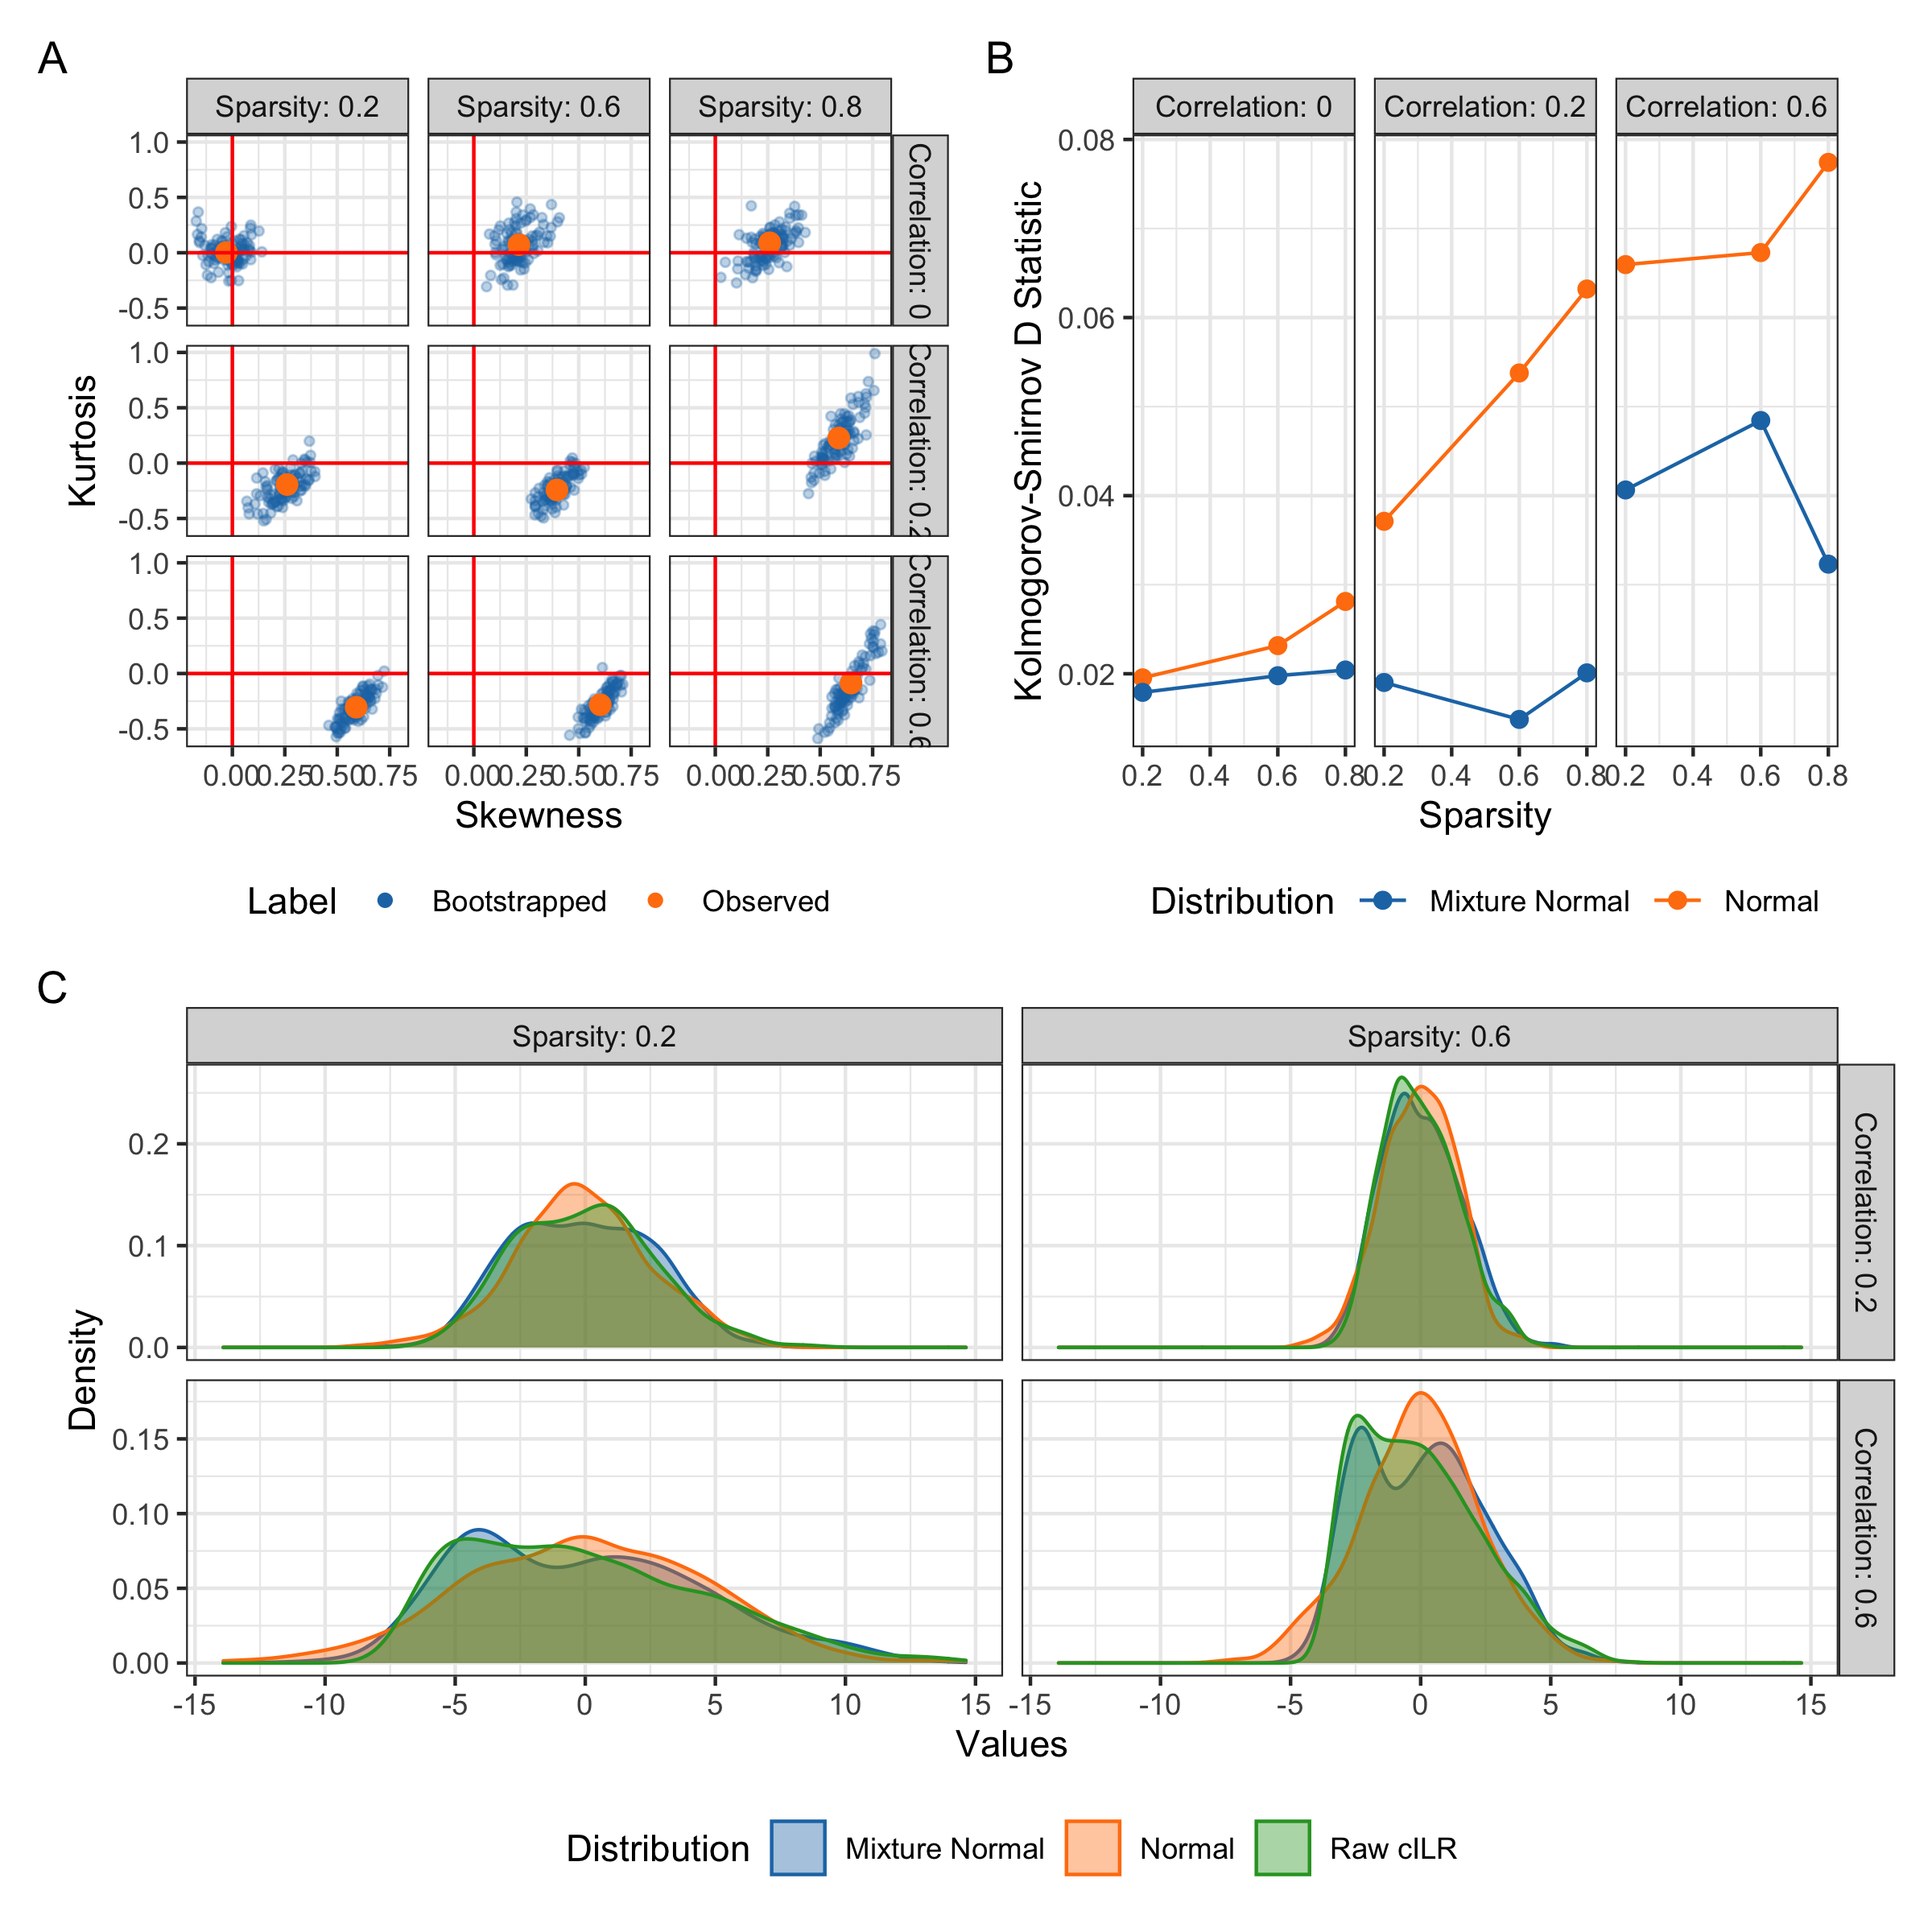
\includegraphics[width=\linewidth]{figures/kurtosis_skewness_gof.png}
    \caption{{\bf Properties of the null distribution of CBEA under the global null simulations}. Panel \textbf{(B)} presents kurtosis and skewness of CBEA scores while panel \textbf{(A)} presents the goodness of fit (as Kolmogorov-Smirnov D statistic) for mixture normal and normal distributions. Panel \textbf{(C)} is a density plot of the shape of the null distribution. Results indicated the necessity of estimating an empirical null and demonstrating that the mixture distribution was the better fit compared to the basic normal.}
    \label{fig:1}
\end{figure}

Additionally, the degree of kurtosis and skewness also suggests that the normal distribution itself might not be a good approximation of the null. To address this issue, we also evaluated a mixture distribution of two normal components. Panel B of Fig~\ref{fig:1} demonstrates the goodness of fit of the mixture normal and the normal distribution using Kolmogorov-Smirnov (KS) test statistic computed on fitted normal and mixture normal distribution when fitted on CBEA scores in simulation scenarios under the global null. We can see that the mixture normal distribution is a better fit (lower KS scores) than the normal distribution across both sparsity and correlation settings. 

We performed our empirical null estimation by fitting our distribution of choice and computing relevant parameters on raw CBEA scores on taxa-permuted data (equivalent to gene permutation in the gene expression literature). As such, the null distribution is characterized by scores computed on sets of equal size with randomly drawn taxa. 

However, null distribution based on taxa-permutation is sensitive to inter-taxa correlations within the set \cite{wu2012}. Since the permutation procedure does not preserve correlation structures, estimating parameters from empirical scores on permuted data will underestimate the variance inflation due to correlation. We account for this by combining the mean estimate from permuted data with the variance estimate from unpermuted data, where the inter-taxa correlation structure remains undisturbed. However, this procedure assumes that the variance of CBEA is equal under both the null and alternate hypotheses. 

\section*{Evaluation}
All code and data sets used for evaluation of this method is publicly available and can be found on GitHub (\href{www.github.com/qpmnguyen/CBEA\_analysis}{qpmnguyen/CBEA\_analysis}). 

\subsection*{Simulation Analysis}
\subsubsection*{Data generation model}  
To address the performance of CBEA for different modeling tasks, we simulated microbiome count data under the assumption that it follows a zero-inflated negative binomial distribution, which is a good fit for real microbiome relative abundance data \cite{calgaro2020}. Suppose $X_{ij}$ are observed counts for a sample $i$ and taxon $j$, then we have the following probability model
\begin{equation}
    \mathbf{X}_{ij} =
      \begin{cases}
        0 & \text{with probability $p_j$}\\
        \mathbf{NB}(\mu_j, \phi_j) & \text{with probability $1 - p_j$}\\
      \end{cases}       
\end{equation}

where $\mu_j$ and $\phi_j$ are mean and dispersion parameters, respectively. To incorporate a flexible correlation structure into our simulation model, we utilized the NorTA (Normal to Anything) method \cite{cario1997}. Given an $n$ by $p$ matrix of values $\mathbf{U}$ sampled from multivariate normal distribution with correlation matrix $\mathbf{\rho}$, we can generate target microbiome count vector $\mathbf{X_{.j}}$ for taxa $j$ following the marginal distribution $\mathbf{NB}$ characterized by the negative binomial cumulative distribution function $\mathbb{F_{\mathbf{NB}}}$:
\begin{equation}
    \mathbf{X}_{.j} = \mathbb{F_{\mathbf{NB}}}^{-1}(\Phi_{U_i})
\end{equation}
In this instance, for each taxon $j$, we set elements in $\mathbf{U}_{.j}$ to be zero with probability $p_j$ and applied $\mathbf{NB}^{-1}(\mu_j, \phi_j)$ on non-zero elements to generate our final count matrix $\mathbf{X}$. To ensure that our simulations match closely to real data, we fitted negative binomial distribution using a maximum likelihood approach (with the \emph{fitdistrplus} package in R \cite{delignette-muller2015}) to non-zero counts for each taxon from 16S rRNA profiling of stool samples from the Human Microbiome Project (HMP). We take the median values of the estimated mean and dispersion parameters as the baseline of our simulations. For simplicity, we assumed that inter-taxa correlation follows an exchangeable structure

\subsubsection*{Simulation scenarios for enrichment analysis at the sample level}
To assess type I error rate and power for enrichment significance testing at the sample level, we simulated data based on the schema above, and assessed enrichment for one focal set. Type I error was obtained under the global null as the number of samples where the null hypothesis was rejected at $\alpha = 0.05$ over the total number of samples (which represents the total number of hypotheses tested). Power was obtained using the same formulation as type I error rate but under the global alternate. We treated type I error and power as estimates of binomial proportions and utilized the Agresti-Couli \cite{agresti1998} formulation to calculate 95\% confidence intervals. Across both analyses, we varied sparsity levels ($p = 0.2, 0.4, 0.6$) and inter-taxa correlation within the set ($\rho = 0, 0.2, 0.5$). For type I error analysis, we also varied the size of the set (50, 100, 150). For power analyses, set size was kept constant at 100 but different effect sizes (fold change of 1.5, 2, and 3). All sample sizes were set at 10,000. 

For classifiability, we evaluated the scores against the true labels per sample (indicating the sample has a set with inflated counts) using the area under the receiving operator curve (AUC). This is a strategy used in Frost \cite{frost2020a} which evaluates the informativeness of scores by assessing the relative ranking of samples (i.e. whether samples with inflated counts are highly ranked using estimated scores).  DeLong 95\% confidence intervals for AUC \cite{delong1988} were obtained for each estimate. Simulation settings for classification performance were identical to power analyses as detailed in the previous paragraph. 

\subsubsection*{Simulation scenarios for enrichment analysis at the population level}
To assess type I error rate and power for differential abundance testing task, we simulated data based on the schema above, and assessed differential abundance of 50 sets with 100 taxa per set across 20 replicates per simulation condition. Type I error is calculated as the number of differentially abundant sets over the total number of sets for each simulation under the global null. Power is defined similarly, but instead under the global alternate hypothesis. Estimates and confidence intervals for type I error and power are calculated as cross-replicate mean and standard error. A set is differentially abundant when all taxa within a set are differentially abundant with the same effect size. Across both analyses, we varied sparsity levels ($p = 0.2, 0.4, 0.6$), and inter-taxa correlation within the set ($\rho = 0, 0.2, 0.5$). Half of the sets are differentially abundant across case/control status with varying effect sizes (fold change of 1.5, 2, and 3). Due to the compositional nature of microbiome taxonomic data, simple inflation of raw counts would cause an artificial decrease in the abundance of the remaining un-inflated sets. As such, we applied a compensation procedure as described in Hawinkel et al. \cite{hawinkel2019} to ensure the validity of simulation results. All sample sizes were set at 2,000.    

\subsubsection*{Simulation scenarios for downstream prediction}
To assess predictive performance, we generated predictors based on the simulation schema presented above and evaluated prediction for both binary and continuous outcomes using a standard random forest model \cite{breiman2001}. For binary outcomes, we use AUC similar to the classification analyses above. For continuous outcomes, we used root mean squared error (RMSE). All predictive model fitting was performed using \emph{tidymodels} \cite{kuhn2020} suite of packages. Across both learning tasks, we varied sparsity ($p = 0.2, 0.4, 0.6$), and inter-taxa correlation ($\rho = 0, 0.2, 0.5$). Continuous outcomes $Y_{cont}$ were generated as linear combinations of taxa counts.  
\begin{equation}
    Y_{cont} = f(\mathbf{X}) + \mathbf{\epsilon}
\end{equation}
where $\mathbf{\epsilon} \sim N(0, \sigma_{\epsilon}^2)$ and $f(\mathbf{X}) = \beta_0 + \mathbf{X}\mathbf{\beta}$. For each simulation, we set $\beta_0$ to be $\frac{6}{\sqrt{10}}$ similar to \cite{xiao2018}. The degree of model saturation (the number of non zero $\mathbf{\beta}$ values) were varied between 0.1 and 0.5, and signal to noise ratio (SNR = $\frac{\sigma(f(\mathbf{X}))}{\sigma_{\epsilon}}$) was varied between 1.5, 2, and 3. 

For binary outcomes, we generate $Y_{binary}$ as Bernoulli draws with probability $p_{binary}$, where 
\begin{equation}
    p_{binary} = \frac{1}{1 + \exp(f(\mathbf{X}) + \mathbf{\epsilon})}
\end{equation}
To ensure a balance of classes, we applied the strategy described in Dong et al. \cite{dong2020} where the associated $\beta$ values are evenly split between positive and negative associations. All data sets generated from prediction tasks have 2,000 samples with 5,000 taxa over 50 sets with a size of 100 taxa per set.  

\subsection*{Evaluation using real data}
In addition to simulation analyses, we also evaluated our method using real data sets based on both 16S rRNA gene sequencing and whole-genome sequencing. We follow the benchmark set by Geistlinger et al. \cite{geistlinger} All data sets are obtained from either the \emph{curatedMetagenomicData} \cite{pasolli2017} and \emph{HMP16SData} \cite{schiffer2019} R packages (2020-10-02 snapshot), or downloaded from the Qiita platform \cite{gonzalez2018}.  

\noindent \textbf{Single Sample Enrichment}: To assess the false discovery rate and true discovery rate of CBEA in sample-level enrichment testing, we utilized the 16S rRNA gene sequencing of the oral microbiome at the gingival subsite from the Human Microbiome Project \cite{consortium2012, proctor2019}. We utilized this data set following the approach outlined in Calagaro et al. \cite{calgaro2020}. This data set is approximately labeled, where aerobic microbes are enriched in the supragingival subsite where the biofilm is exposed to the open air, while conversely anaerobic microbes thrive in the subgingival site \cite{thurnheer2016}. Here, we assessed the enrichment of aerobic microbes across all samples, we considered the false positive rate as the number of samples from the subgingival site with significant enrichment, and the true positive rate as the number of supragingival samples with significant enrichment. Microbial tropism annotation at the genus level was from Beghini et al. \cite{beghini2019} and was downloaded directly from the GitHub repository associated with Calagaro et al. \cite{matteocalgaro2020}. 

\noindent \textbf{Differential Abundance Analsysis}: To assess type I error using CBEA scores in differential abundance analysis, we utilized the 16S rRNA gene sequencing of stool samples from the Human Microbiome Project \cite{consortium2012, proctor2019}. Here, we randomly assign samples a label of case or control, and repeated this process 500 times, assessing all candidate methods at each iteration. Type I error is then the number of taxa identified as differentially abundant across all tested taxa. For the true positive rate, we used the same gingival data set as described above. However, instead of testing for aerobic microbes as a group, the true positive rate is the number of aerobic/anaerobic genera identified as differentially abundant across all aerobic or anaerobic genera. 

\noindent \textbf{Disease Prediction}: To assess predictive power, we utilized the whole genome sequencing of stool samples of inflammatory bowel disease (IBD) patients from the MetaHIT consortium \cite{nielsen2014}. This data set contains 396 samples from a cohort of European adults, where 195 adults were classified as having IBD (which includes patients diagnosed with either ulcerative colitis or Crohn's disease). Additionally, we also utilized a similar data set from Gevers et al. \cite{gevers2014} which also profiles the gut microbiome of IBD patients and controls but using 16S rRNA gene sequencing. This data set contains 16S rRNA gene sequencing samples from a cohort of pediatric patients (ages $<$ 17) from the RISK cohort enrolled in the United States and Canada. Of the 671 samples obtained, 500 samples belong to patients with IBD. 

\subsubsection*{Comparison Methods}

\noindent \textbf{Single sample enrichment}: For type I error and power analyses, we compared the CBEA method with a naive Wilcoxon rank sum test. We added a pseudocount of 1 to all values. This is a non-parametric difference in means test, where we compared the abundance of taxa of a pre-defined set and its complement within a single sample. For classification performance, we compared CBEA methods against GSVA \cite{hanzelmann2013}, ssGSEA \cite{barbie2009}, and the W-statistic from the Wilcoxon rank sum test. All three approaches were applied directly on count data (after pseudocount). For GSVA, the Poisson kernel was used. 

\noindent \textbf{Differential Abundance}: Since CBEA are sample-level enrichment scores, we performed differential abundance by using a Wilcoxon Rank Sum test and Welch's t-test across case/control status on CBEA generated scores. We added a pseudocount of 1 to all values. For comparison, we chose representative state-of-the-art methods in differential abundance analysis, namely DESeq2 \cite{love2014,mcmurdie2014} and corncob \cite{martin2020}. For DESeq2, we performed a likelihood ratio test against an intercept only reduced model with dispersion estimated with local fit. For corncob, we also performed a likelihood ratio test against an intercept only reduced model without bootstrapping. 

\noindent \textbf{Disease Prediction}: We fit random forest on CBEA scores, as well as ssGSEA \cite{hanzelmann2013} and GSVA \cite{barbie2009} similar to single sample enrichment section. We added a pseudocount of 1 to all values. Additionally, we also compared performance using CBEA against a standard analysis plan where the centered log-ratio transformation (CLR) was applied to count-aggregated sets as inputs to a machine learning model. 

\section*{Results}
In this section, we present the performance of our proposed method for three applicable microbiome analysis tasks: sample level enrichment, differential abundance, and disease prediction. We obtained these results from both parametric simulations and examples from real data.  

\subsection*{Enrichment testing at the sample level}
CBEA provides significance testing for enrichment at the sample level using the null distribution estimation procedure described in \nameref{methods}. Here, we present empirical results for this application of CBEA assessing type I error, power, and classification capacity. 

\subsubsection*{Simulation studies}
Panel A and B in Fig~\ref{fig:2} demonstrate type I error and power respectively across different simulation conditions. We benchmarked the results of the CBEA method against a naive Wilcoxon rank sum test performed at the sample level, comparing the mean count difference between taxa in the set its complement. All methods demonstrate good type I error control at $\alpha = 0.05$ under zero correlation across all simulation conditions. However, under both medium ($\rho = 0.2$) and high ($\rho = 0.5$) correlation settings, both the Wilcoxon test and unadjusted CBEA variants show high levels of inflated type I error, where Wilcoxon test performed the worst. On the other hand, adjusted CBEA methods (under both distributions) control for type I error at the appropriate $\alpha$ level even at high correlations. 

\begin{figure}[!h]
    \centering
    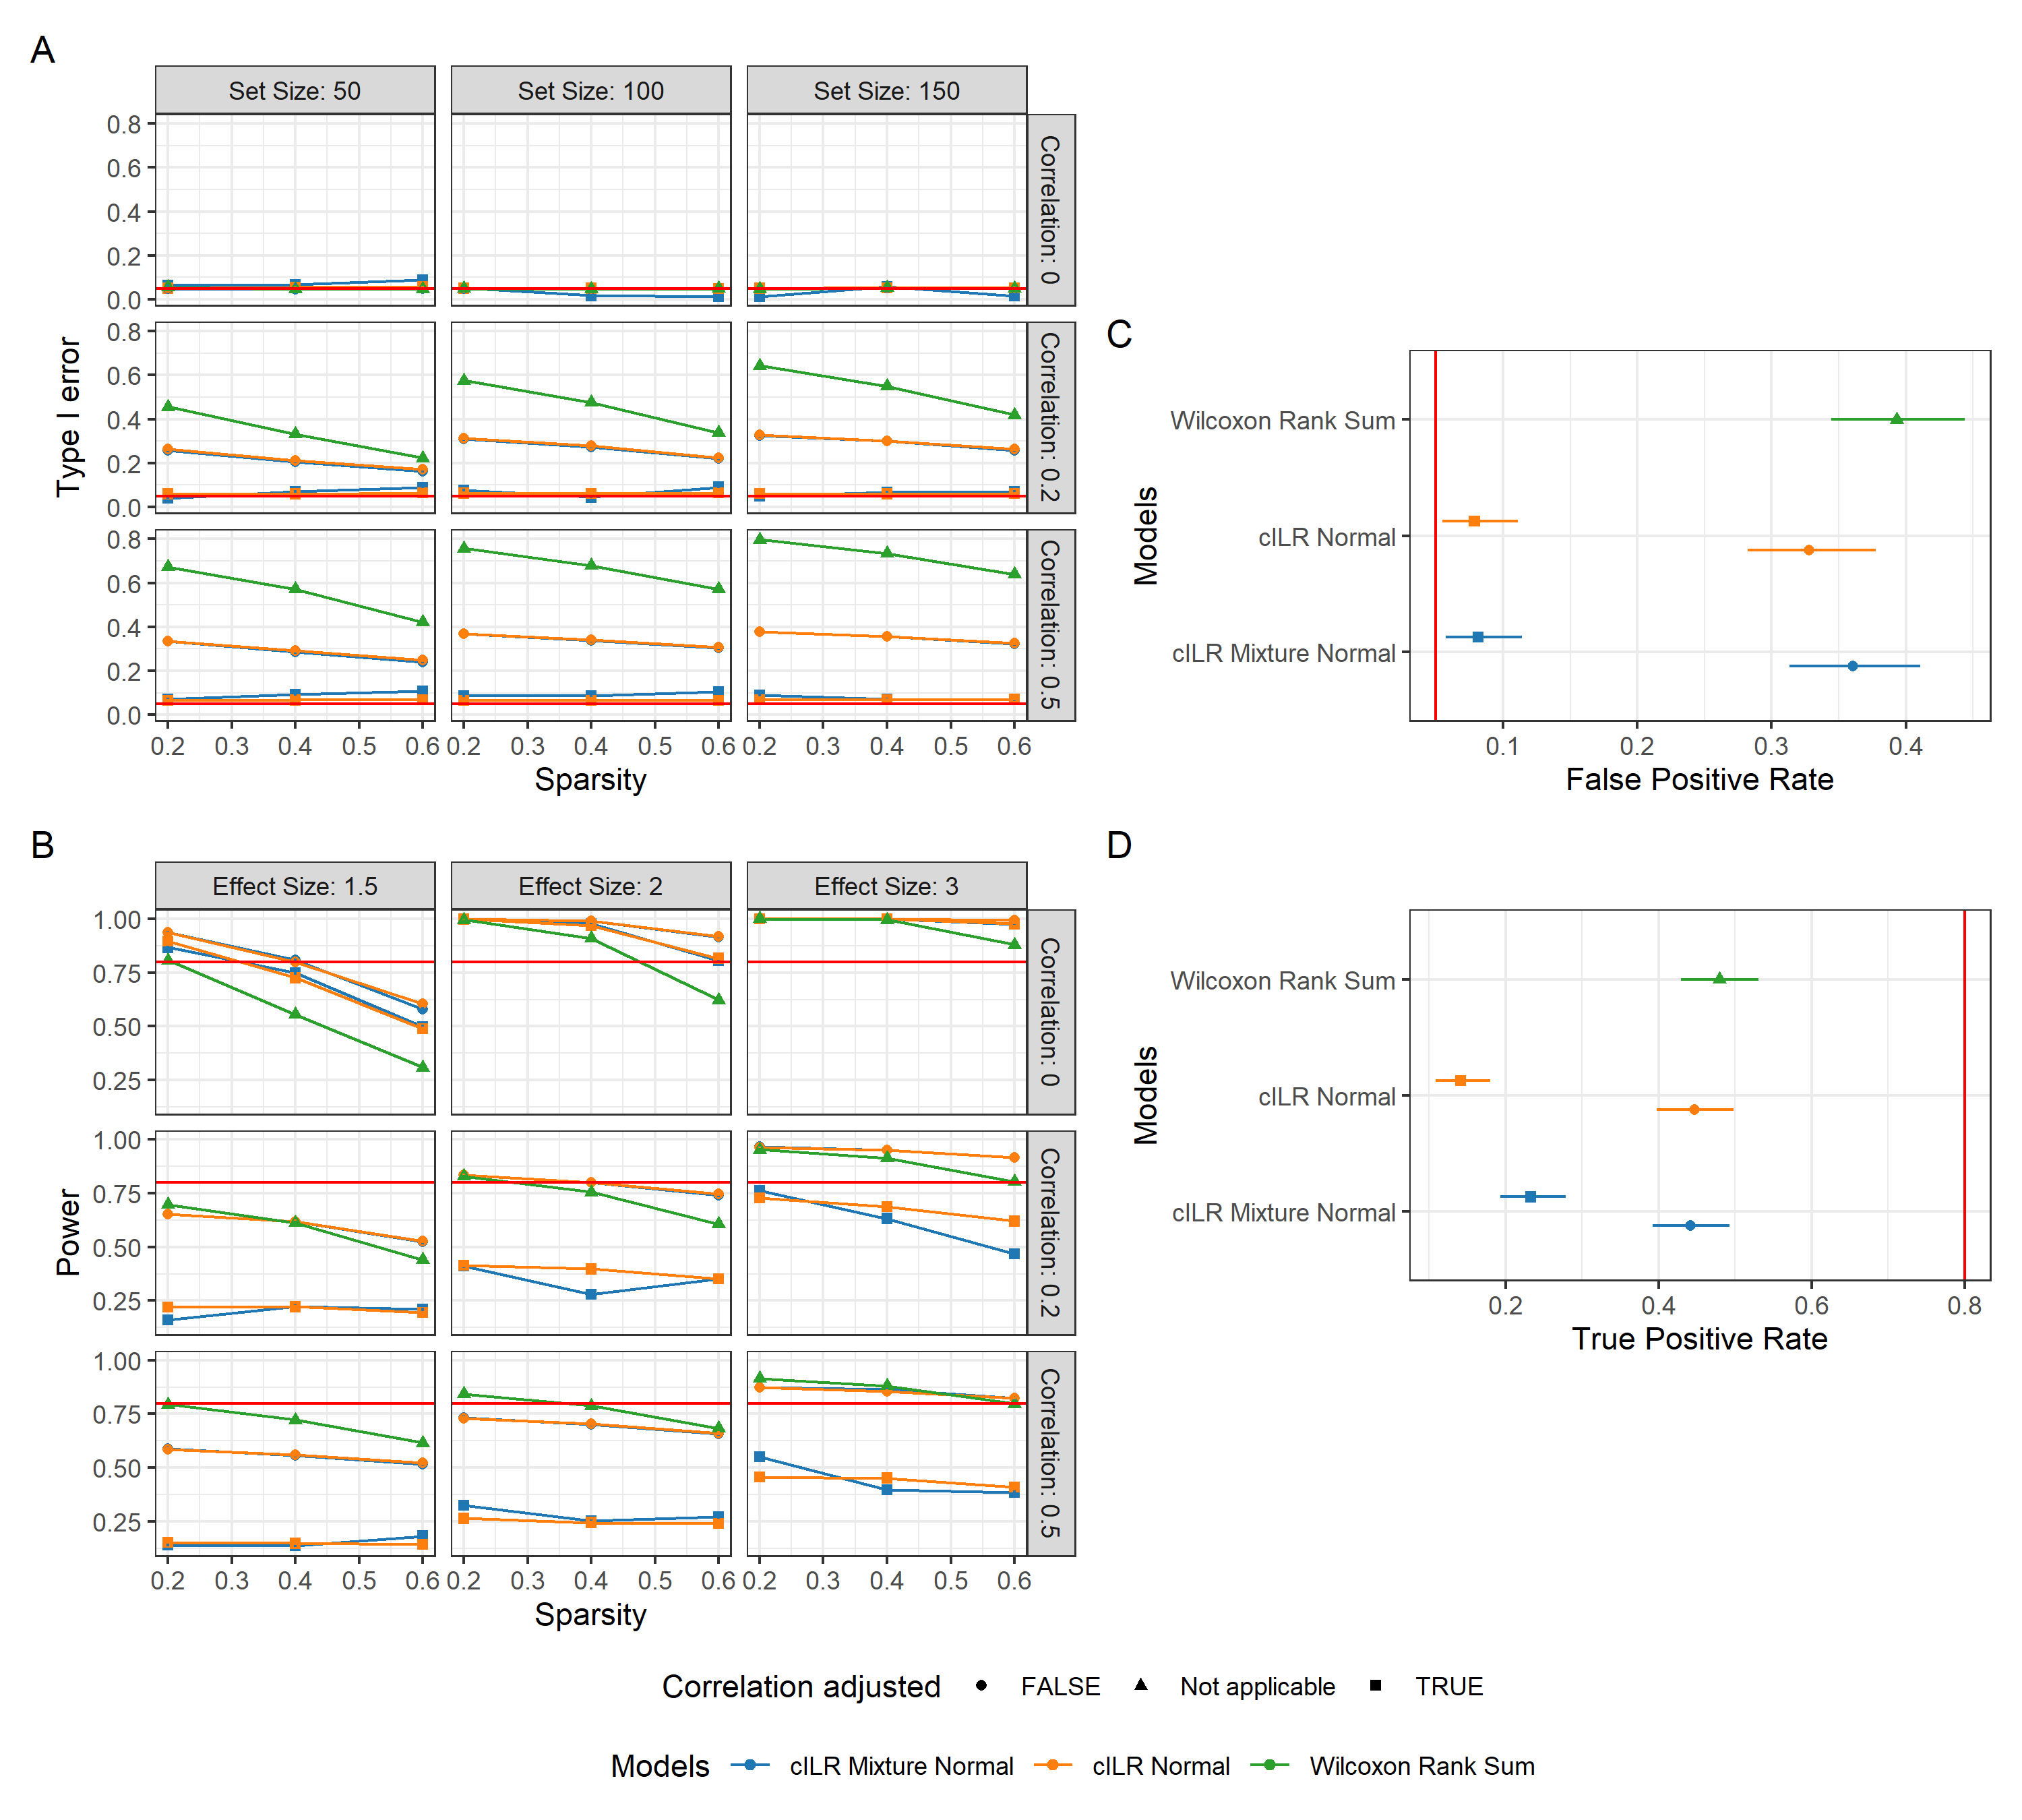
\includegraphics[width=\textwidth]{figures/sim_data_ss_hypo.png}
    \caption{Sample-level inference with CBEA under parametric simulations (\textbf{(A)} and \textbf{B}), and real data analysis (\textbf{(C)} and \textbf{(D)}). In simulation analyses, panel \textbf{(A)} shows type I error rate, and panel \textbf{(B)} shows power for single sample enrichment test for a specified set and was compared against a Wilcoxon rank sum test at $\alpha$ of 0.05. In real data analysis, panel \textbf{(C)} shows the false-positive rate, and panel \textbf{(D)} shows the true positive rate. For this analysis, 16S rRNA data from the oral microbiome of the gingival site was used. The set of aerobic microbes was tested for enrichment in all samples and was identified as correctly enriched if a significant $p$-value was obtained in supragingival samples. Confidence bounds were obtained using Agresti-Couli \cite{agresti1998} approach. Adjusted CBEA demonstrated control of type I error at the appropriate $\alpha$ level while remaining methods (not included in subsequent power analyses) showed an inflated type I error rate. However, this resulted in lower power for adjusted CBEA methods.}
    \label{fig:2}
\end{figure}

However, the trade-off for good type I error control is demonstrably lower power, as shown in Fig~\ref{fig:2}B. In situations where there is no inter-taxa correlation, CBEA still outperforms the wilcoxon rank sum test, however adjusted versions of CBEA did not perform as well as un-adjusted ones. However, in higher correlation scenarios, the difference in power is much more dramatic. At the highest effect size (fold change of 3) and correlation ($\rho = 0.5$), adjusted CBEA was only performing at 50\% power, while unadjusted CBEA and wilcoxon rank sum test were able to reach 80\%. These results indicate that both sparsity and inter-taxa correlation impacts power, with correlation having a much more dramatic impact especially for adjusted versions of CBEA. Most importantly, CBEA demonstrate higher power in all scenarios where type I error is properly controlled.    

To further assess the utility of CBEA in classifying samples with enriched sets, we generated AUC scores for different CBEA scores using true labels of whether a sample has an inflated set. This analysis, therefore, assessed the relative ranking of samples using CBEA scores whereby high scores should correspond to samples that are known to be inflated. Fig~\ref{fig:3} presents this result. We compared different variants of CBEA against competing methods in the gene set testing space (GSVA \cite{hanzelmann2013} and ssGSEA \cite{barbie2009}), as well as the $W$ test statistic from the Wilcoxon rank sum test. Across both simulations (Fig~\ref{fig:3}A) and real-data applications (Fig~\ref{fig:3}B), CBEA scores perform marginally better especially in low effect size situations but did not stand out in most other scenarios. In simulation studies, classification performance was good (around AUC of 0.8) even at high correlation settings, only requiring medium effect sizes (fold change of 2). Notably, the W-statistic provided the least information for classifying samples with inflated taxa.

\subsubsection*{Real data evaluations}  
These observations were replicated when assessed on the semi-labeled gingival data set from the Human Microbiome Project as described in \nameref{methods}. Here, we tested the enrichment of aerobic microbes for each sample using approaches similar to our parametric simulations. As expected in Fig~\ref{fig:2}C, the proportion of falsely rejected hypotheses was high in the naive Wilcoxon test and unadjusted CBEA methods. Conversely, adjusted CBEA controls for false positives adequately at the correct $\alpha$ level of 0.05. Power analysis (Fig~\ref{fig:2}D) showed similar patterns, where unadjusted CBEA methods and the Wilcoxon test have a higher proportion of null hypotheses correctly rejected, however, these results are not useful to a practitioner as the number of falsely rejected hypotheses are also equally high.  

\begin{figure}[!h]
    \centering
    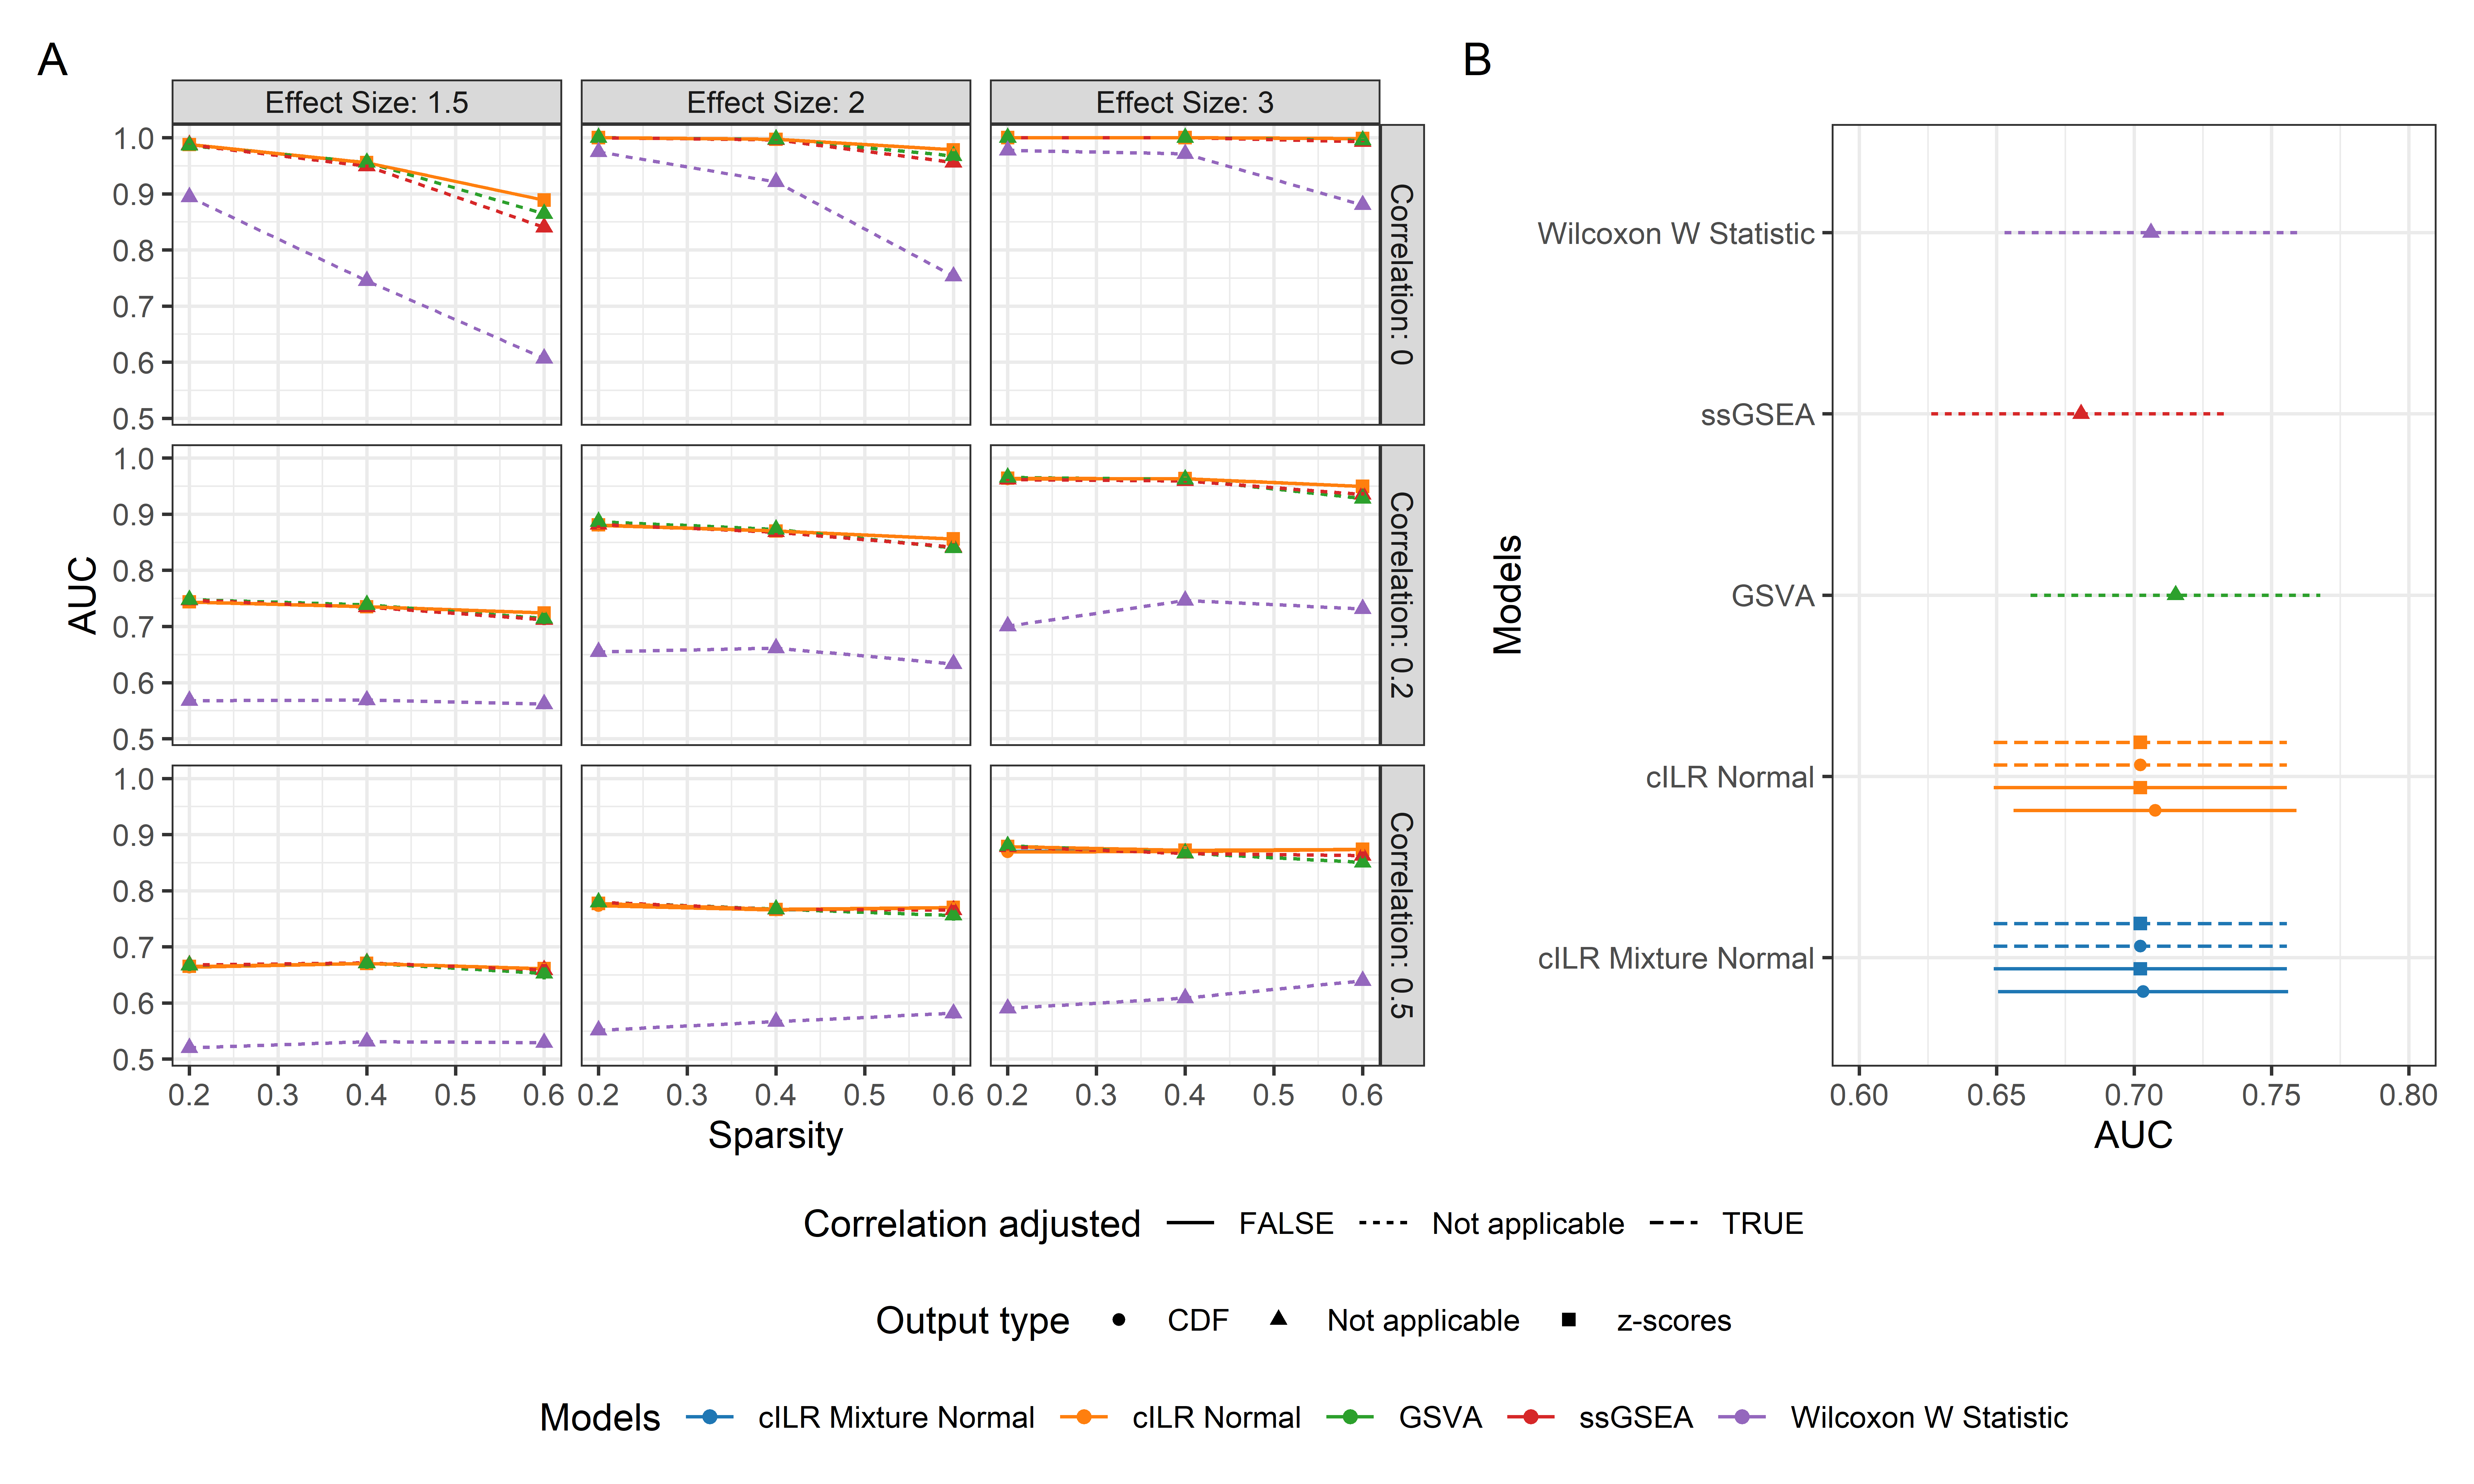
\includegraphics[width = \textwidth]{figures/sim_data_ss_auc.png}
    \caption{Classification performance via AUC of CBEA, ssGSEA, GSVA, and Wilcoxon $U$ statistic on simulated data \textbf{(A)} the gingival data set from the Human Microbiome Project  \textbf{(B)} as detailed in \nameref{methods}. Performance scores measure whether scores can highly rank samples that are known to have inflated abundance. In the gingival data set presented in panel \textbf{(B)}, samples from the supragingival site are assumed to have an inflated abundance of aerobic microbes. Error bars are the 95\% DeLong confidence intervals for AUC \cite{delong1988}} 
    \label{fig:3}
\end{figure}

\subsection*{Differential abundance analysis}
CBEA generates sample-specific scores representing the degree of enrichment of a pre-defined set. As such, we want to assess the ability to use these scores for differential abundance analysis in combination with a standard difference of means statistical test (Welch's t-test and Wilcoxon rank sum test). We compared the performance of this approach with CBEA and two commonly used methods for differential abundance testing in the microbiome literature: DESeq2 \cite{love2014} and corncob \cite{martin2020}.   

\subsubsection*{Simulation studies}
\begin{figure}[!h]
    \centering
    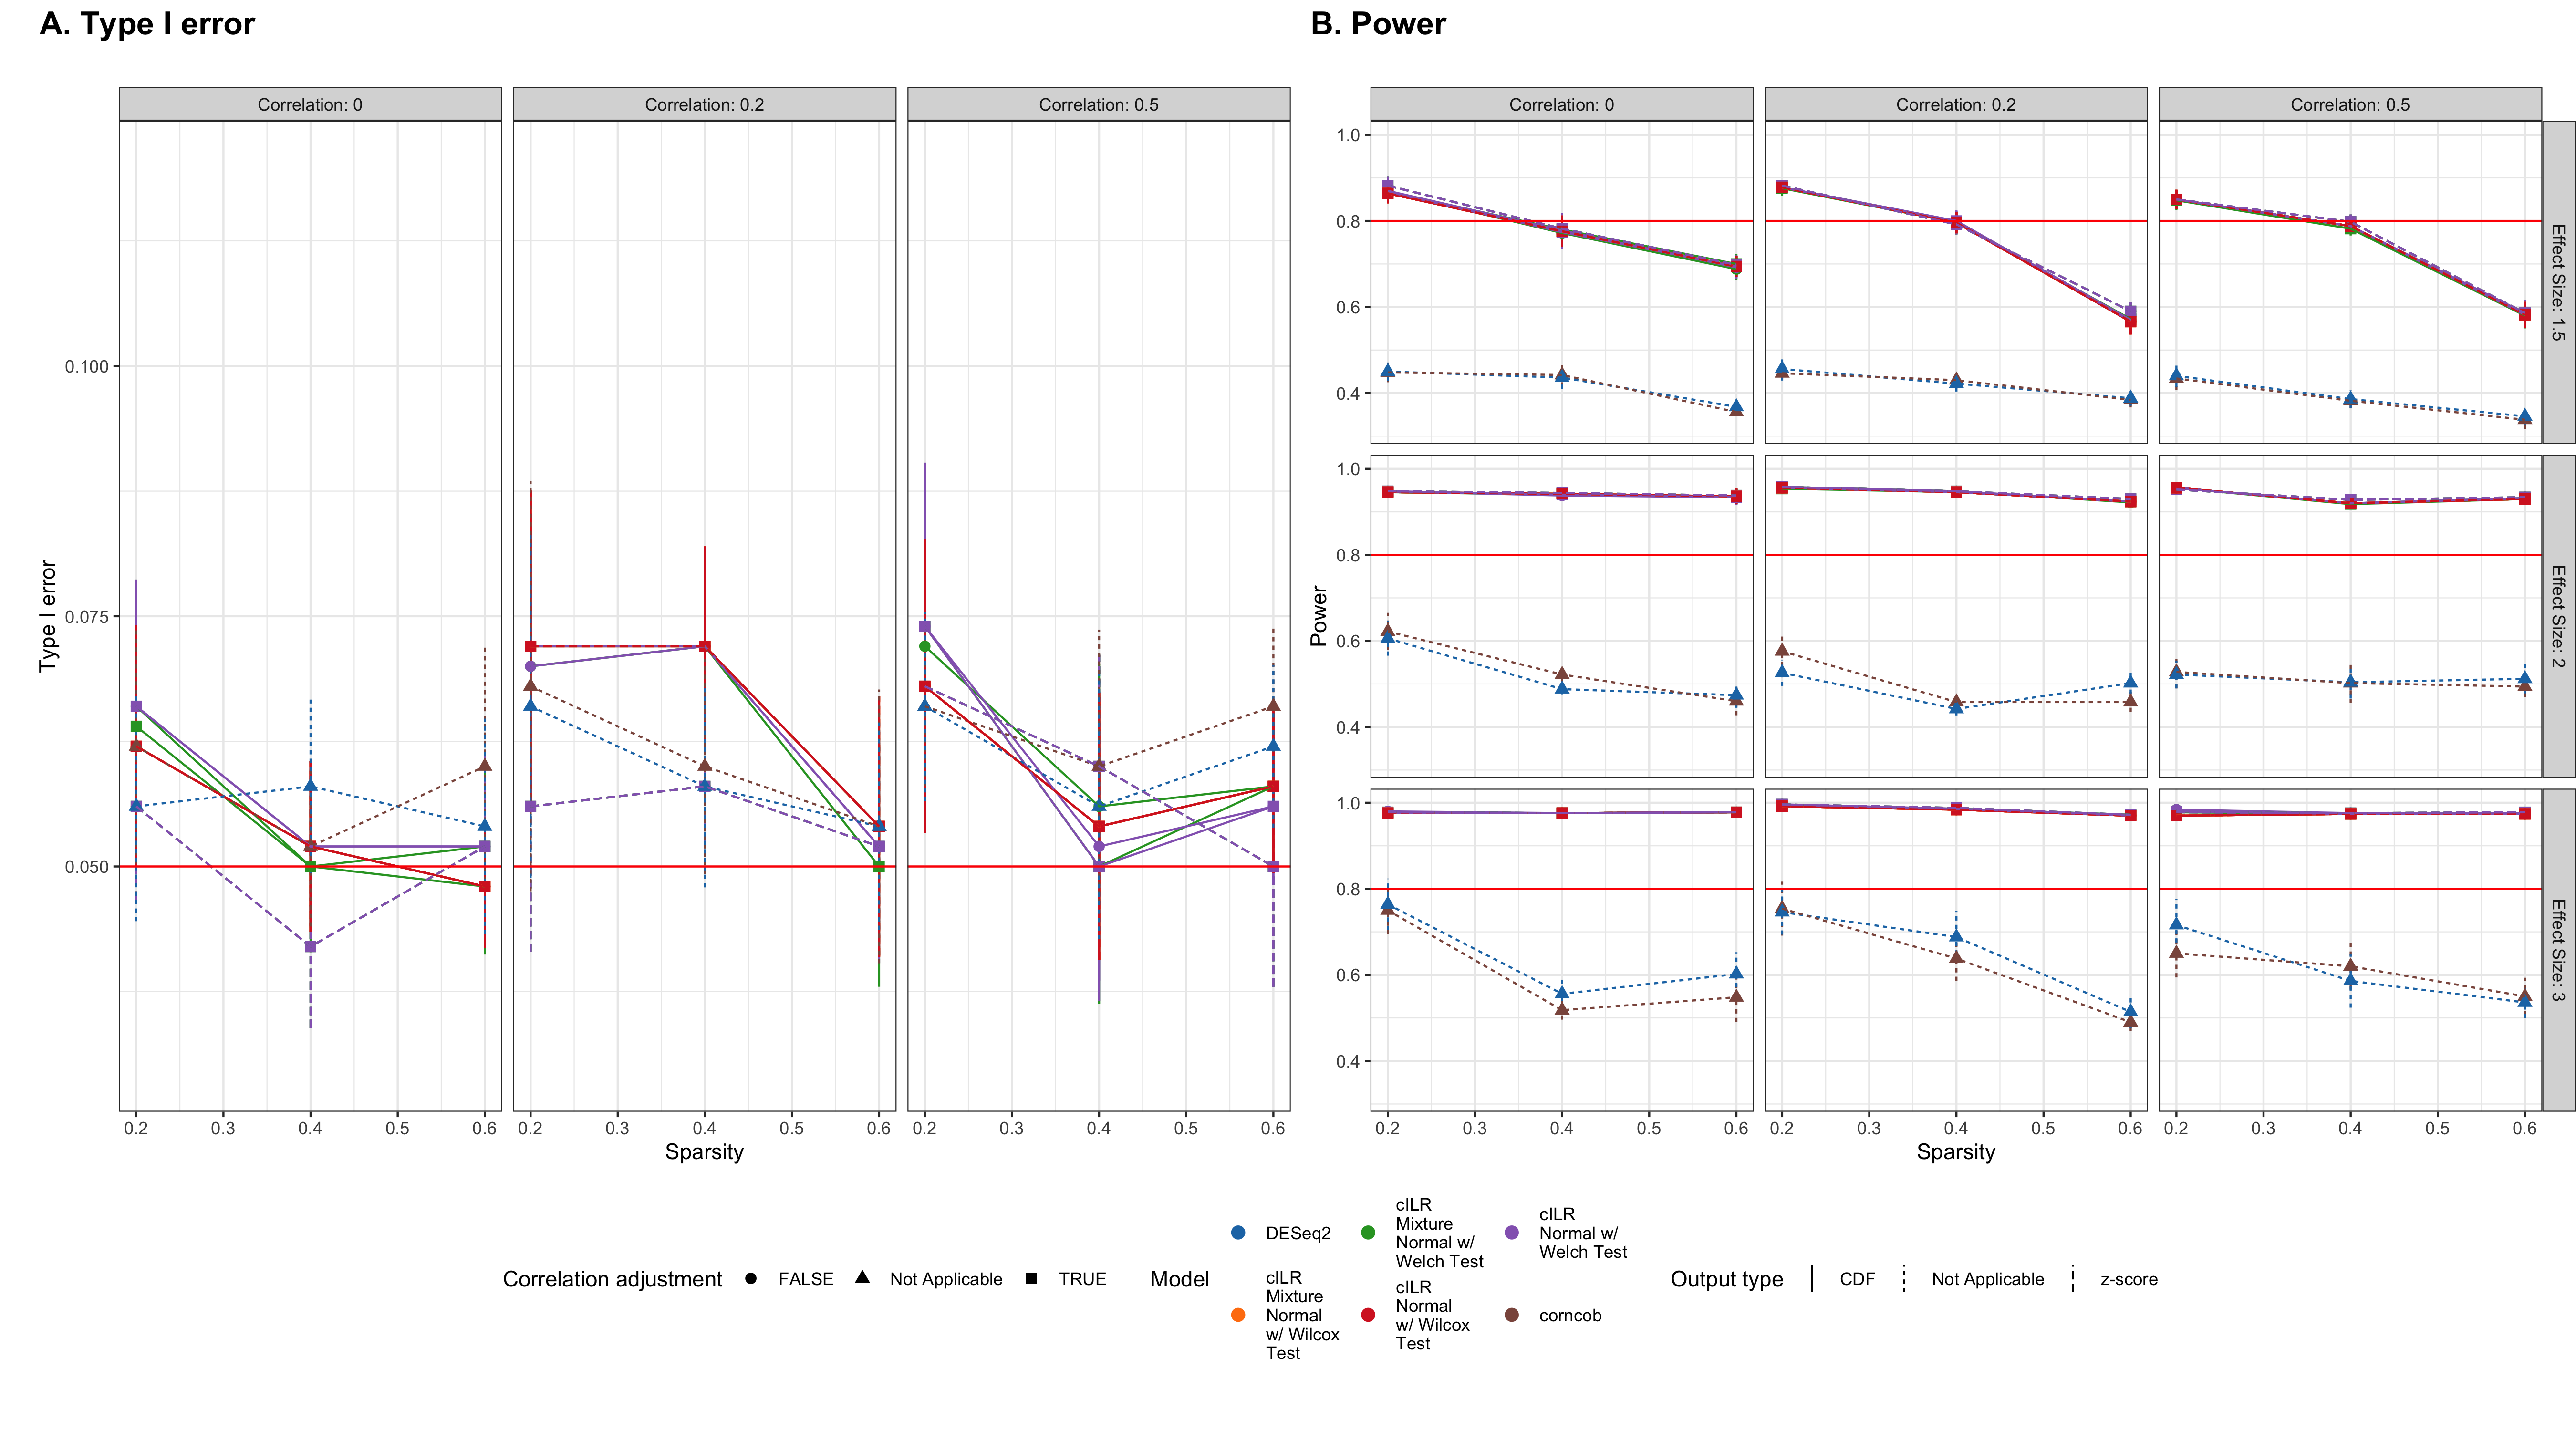
\includegraphics[width = \textwidth]{figures/sim_diff_ab_comb.png}
    \caption{Type I error rate \textbf{(A)} and power \textbf{(B)} for differential abundance test across different parametric simulation scenarios. For CBEA methods, differential abundance analysis was performed using a difference in means test (either Wilcoxon rank-sum test or Welch's t-test) across case/control status using single sample scores generated by CBEA (across different output types and distributional assumptions). CBEA associated methods demonstrated similar type I error to conventional differential abundance analysis methods but with more power to detect differences even at small effect sizes.} 
    \label{fig:4}
\end{figure}

Fig.~\ref{fig:4} present results for simulation studies for both type I error (panel A) and power (panel B) evaluations. All methods control for type I error well across both sparsity and correlation levels, where the estimated rate was consistently around the 0.05 pre-defined threshold. Results were similar across all evaluated methods, although in some instances, for example in medium correlation setting ($\rho = 0.2$), the unadjusted CBEA resulted in higher type I error, regardless of difference in means test and distribution of choice. 

The difference between the methods is more noticeable when evaluating power. All CBEA associated variants showed much higher power even when the effect size is limited (fold change is 1.5), and there is a noticeable gap in performance between CBEA and both DESeq2 and corncob. Surprisingly, this effect is consistent across correlation levels and sparsity, even though we expectedly see performance in power drop as a function of sparsity especially in low effect size settings.  

\subsubsection*{Real data evaluations}
In addition to simulation studies, we also evaluated performance of the methods on real 16S rRNA gene sequencing data set from HMP (Fig~\ref{fig:5}). For type I error evaluations, we use stool samples and randomly assign them with case/control status and calculated type I error as the proportion of genera identified as significantly different. For true positive rate evaluations, we use the gingival data set as detailed in the previous section, and calculated the true positive rate as the proportion of genera labeled as either anaerobic or aerobic that were found to be significant.   

We observed both corncob and DESeq2 had significantly inflated type I error rate while all variations of CBEA were controlling for type I error at the defined $\alpha$ threshold of 0.05. This is surprising given the consistency of preserving type I error for both corncob and DESeq2 in all simulation evaluations. 

In true positive experiments with data from the gingival site, estimated rates were more similar across the different methods. As expected, using the Wilcoxon rank sum test resulted in lower true positive rate compared to remaining methods, but the difference was not noticable. This is also surprising given that in simulation studies, both corncob and DESeq2 showed markedly lower power across all effect sizes.  

\begin{figure}[!h]
    \centering
    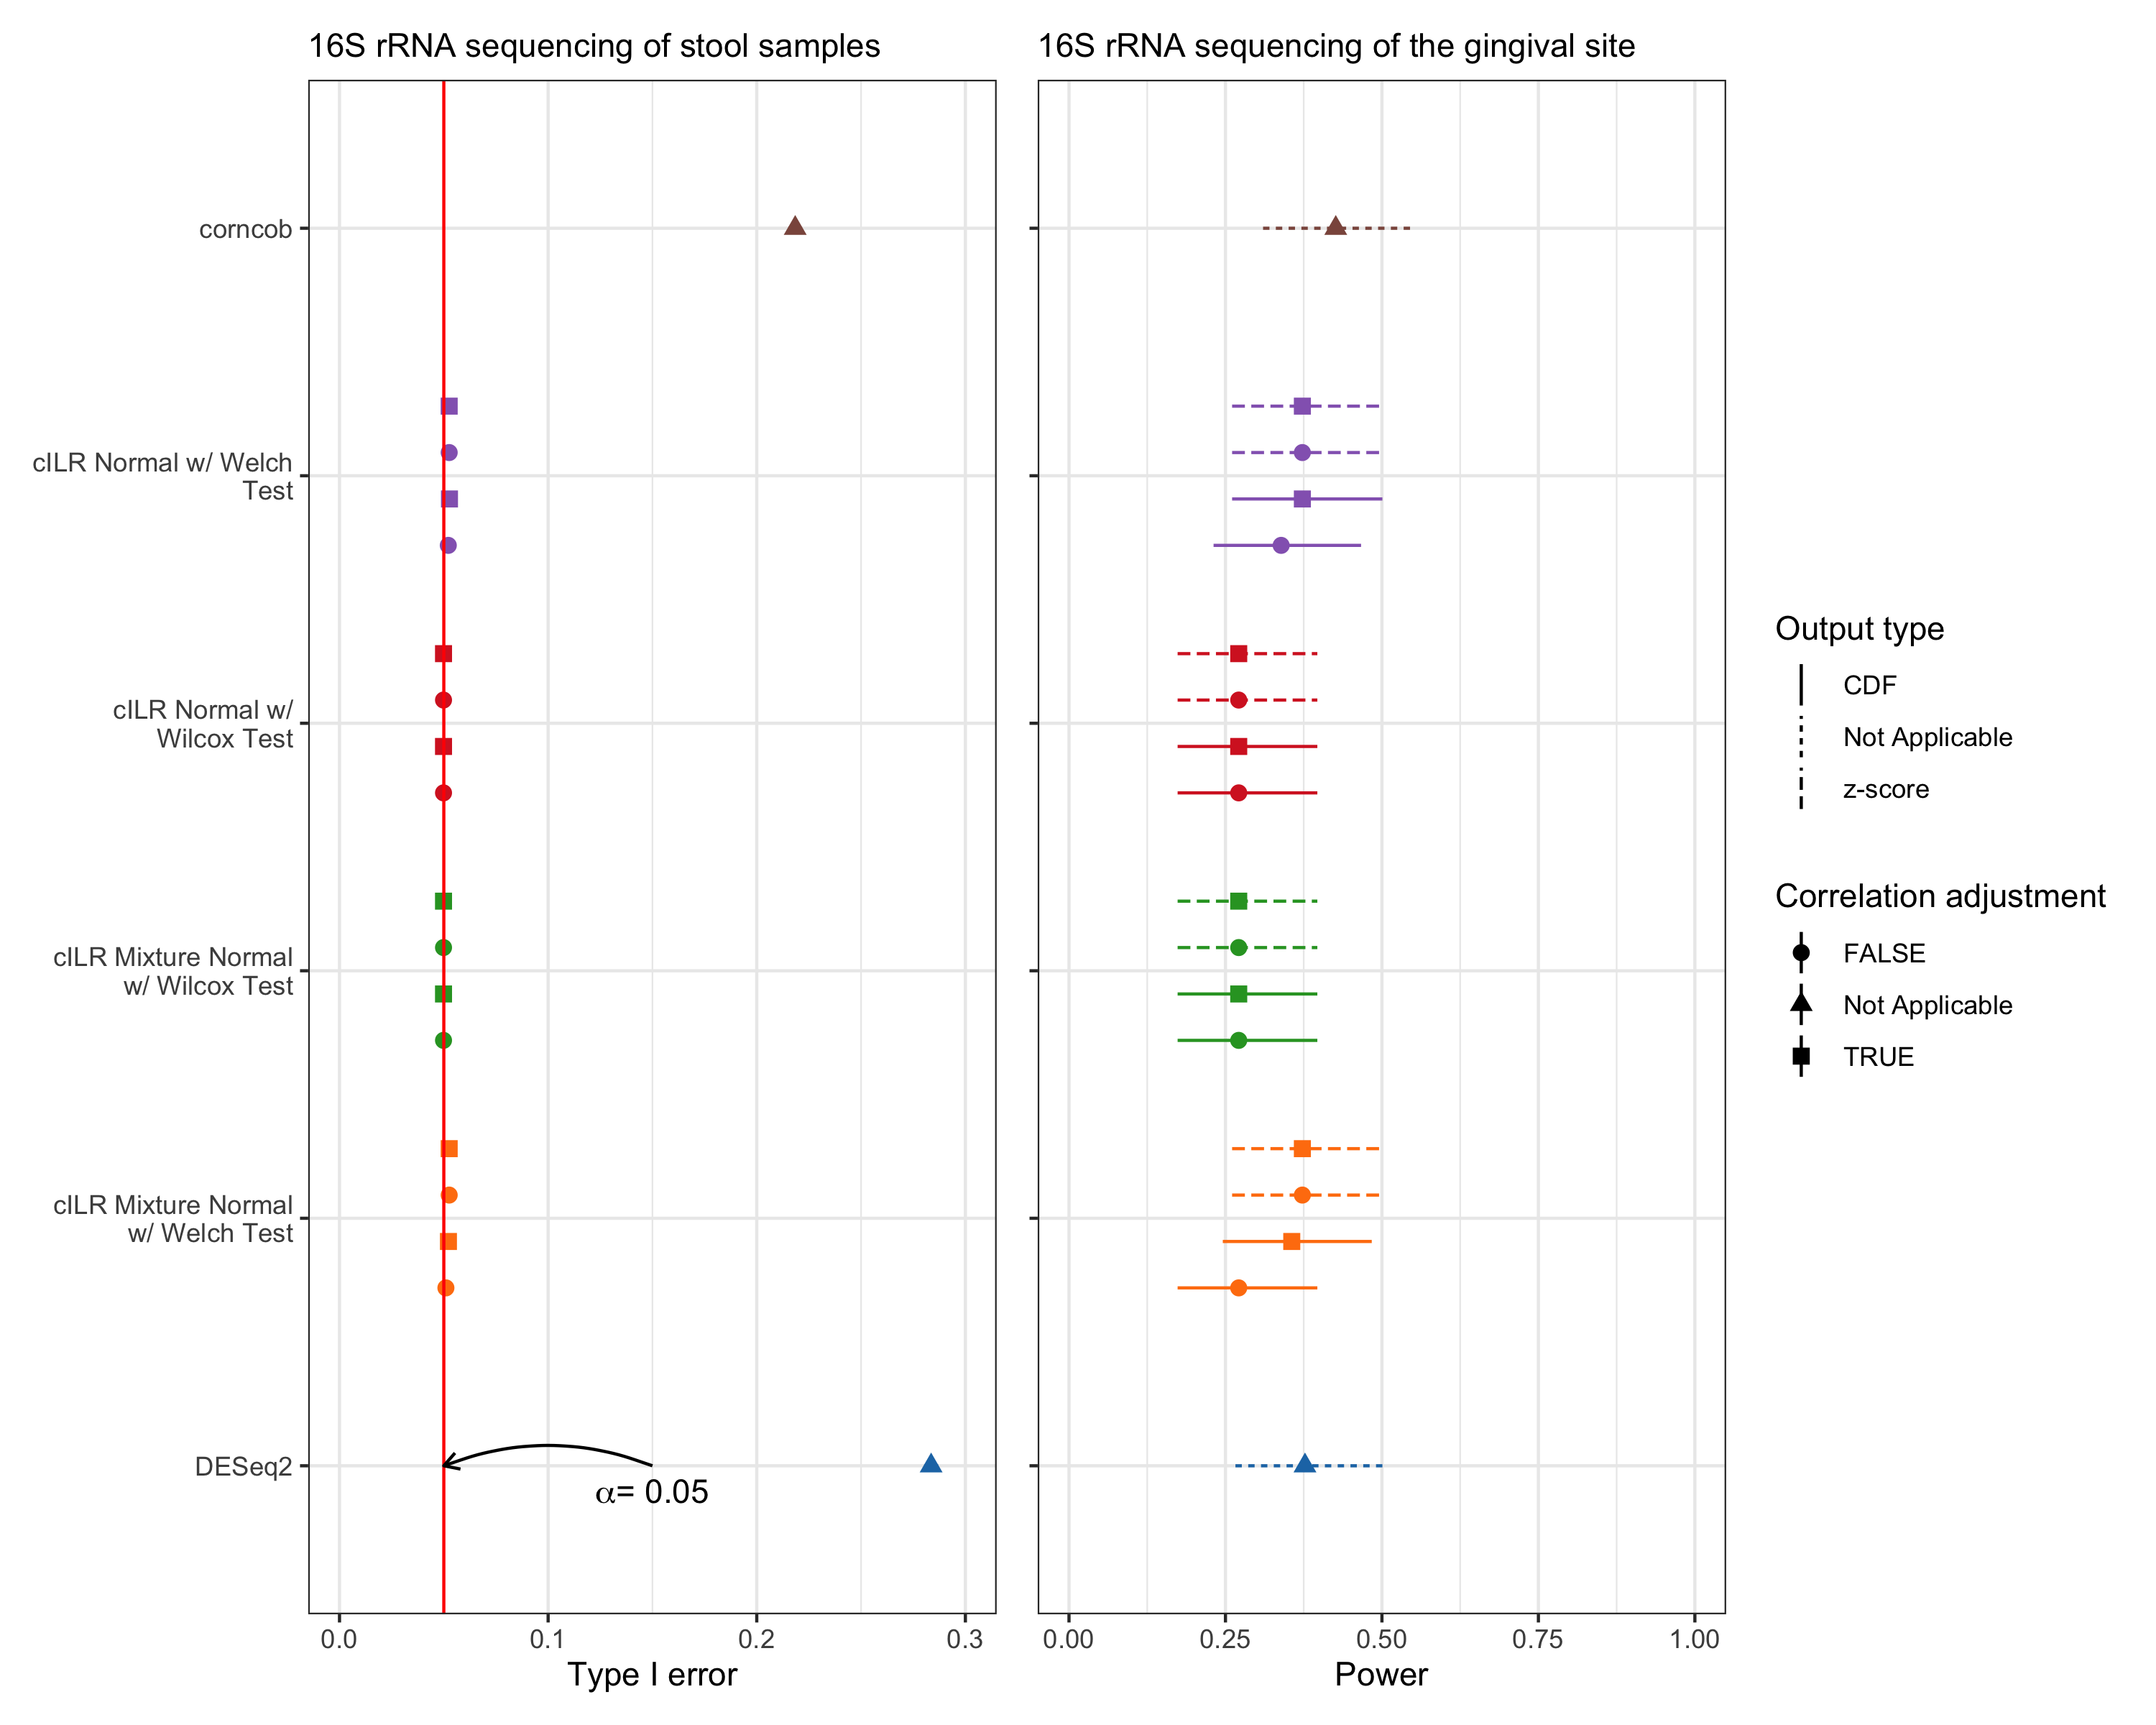
\includegraphics[width = \textwidth]{figures/data_diff_ab.png}
    \caption{Differential abundance analysis using corncob, DESeq2 and CBEA with either Wilcoxon rank sum test or Welch's t-test. Panel \textbf{(A)} shows type I error results as the proportion of significant genera after 500 iterations where case/control status was assigned randomly to each sample. Panel \textbf{(B)} shows true positive rate results as the proportion of significant genera who are either obligate anaerobes or aerobes. Both evaluations use 16S rRNA gene sequencing data from HMP. Type I error evaluation used stool samples while the true positive rate evaluation used samples from the gingival site. Results showed that CBEA associated methods were able to keep type I error rate at approximately 0.05 while still demonstrating similar power as both corncob and DESeq2} 
    \label{fig:5}
\end{figure}

\subsection*{Disease Prediction}   
Since CBEA can generate informative scores that can discriminate between samples with inflated counts for a set (Fig~\ref{fig:2}), we want to assess whether they can also act as useful inputs to predictive models. In this section we assessed the predictive performance of a naive random forest model \cite{breiman2001} with different single sample enrichment scoring methods as inputs (evaluating CBEA, ssGSEA, and GSVA). Additionally, we also compared predictive performance of using these scores against the a standard approach of using the centered log ratio transformation (CLR) on taxon sets aggregated via abundance summations.     
\subsubsection*{Simulation studies}
Fig~\ref{fig:6} shows results for simulation studies as detailed in the \nameref{methods} section. Panel A presents results for a regression learning task with a continuous outcome while panel B presents results for a classification task with a binary outcome. As expected, performance across all assessed methods increased with a higher signal-to-noise ratio. Both CLR and CBEA approaches outperformed both GSVA and ssGSEA across all simulation conditions and learning tasks. This is because both GSVA and ssGSEA are more sensitive to the degree of inter-taxa correlation and sparsity, while CBEA and CLR did not experience a similar level of impact. As such, performance gap widens with increasing correlation and sparsity. Interestingly, this difference in performance is not as pronounced under high levels of effect saturation (across both learning tasks), suggesting that when there is a high number of sets contributing to an effect, model choice might not be as important.   

In this analysis, CBEA unfortunately did not outperform the CLR approach, which is standard practice within the microbiome literature \cite{gloor2017}. This difference in performance is more notable in regression learning tasks compared to classification, and at lower levels of effect saturation. However, the degree of separation between the two approaches is not as dramatic as between GSVA/ssGSEA and CBEA/CLR. Moreover, the performance gap decreases with increasing effect signal-to-noise ratio and sparsity. Additionally, we did not observe any performance difference between the different variations of CBEA. 

\begin{figure}[!h]
    \centering
    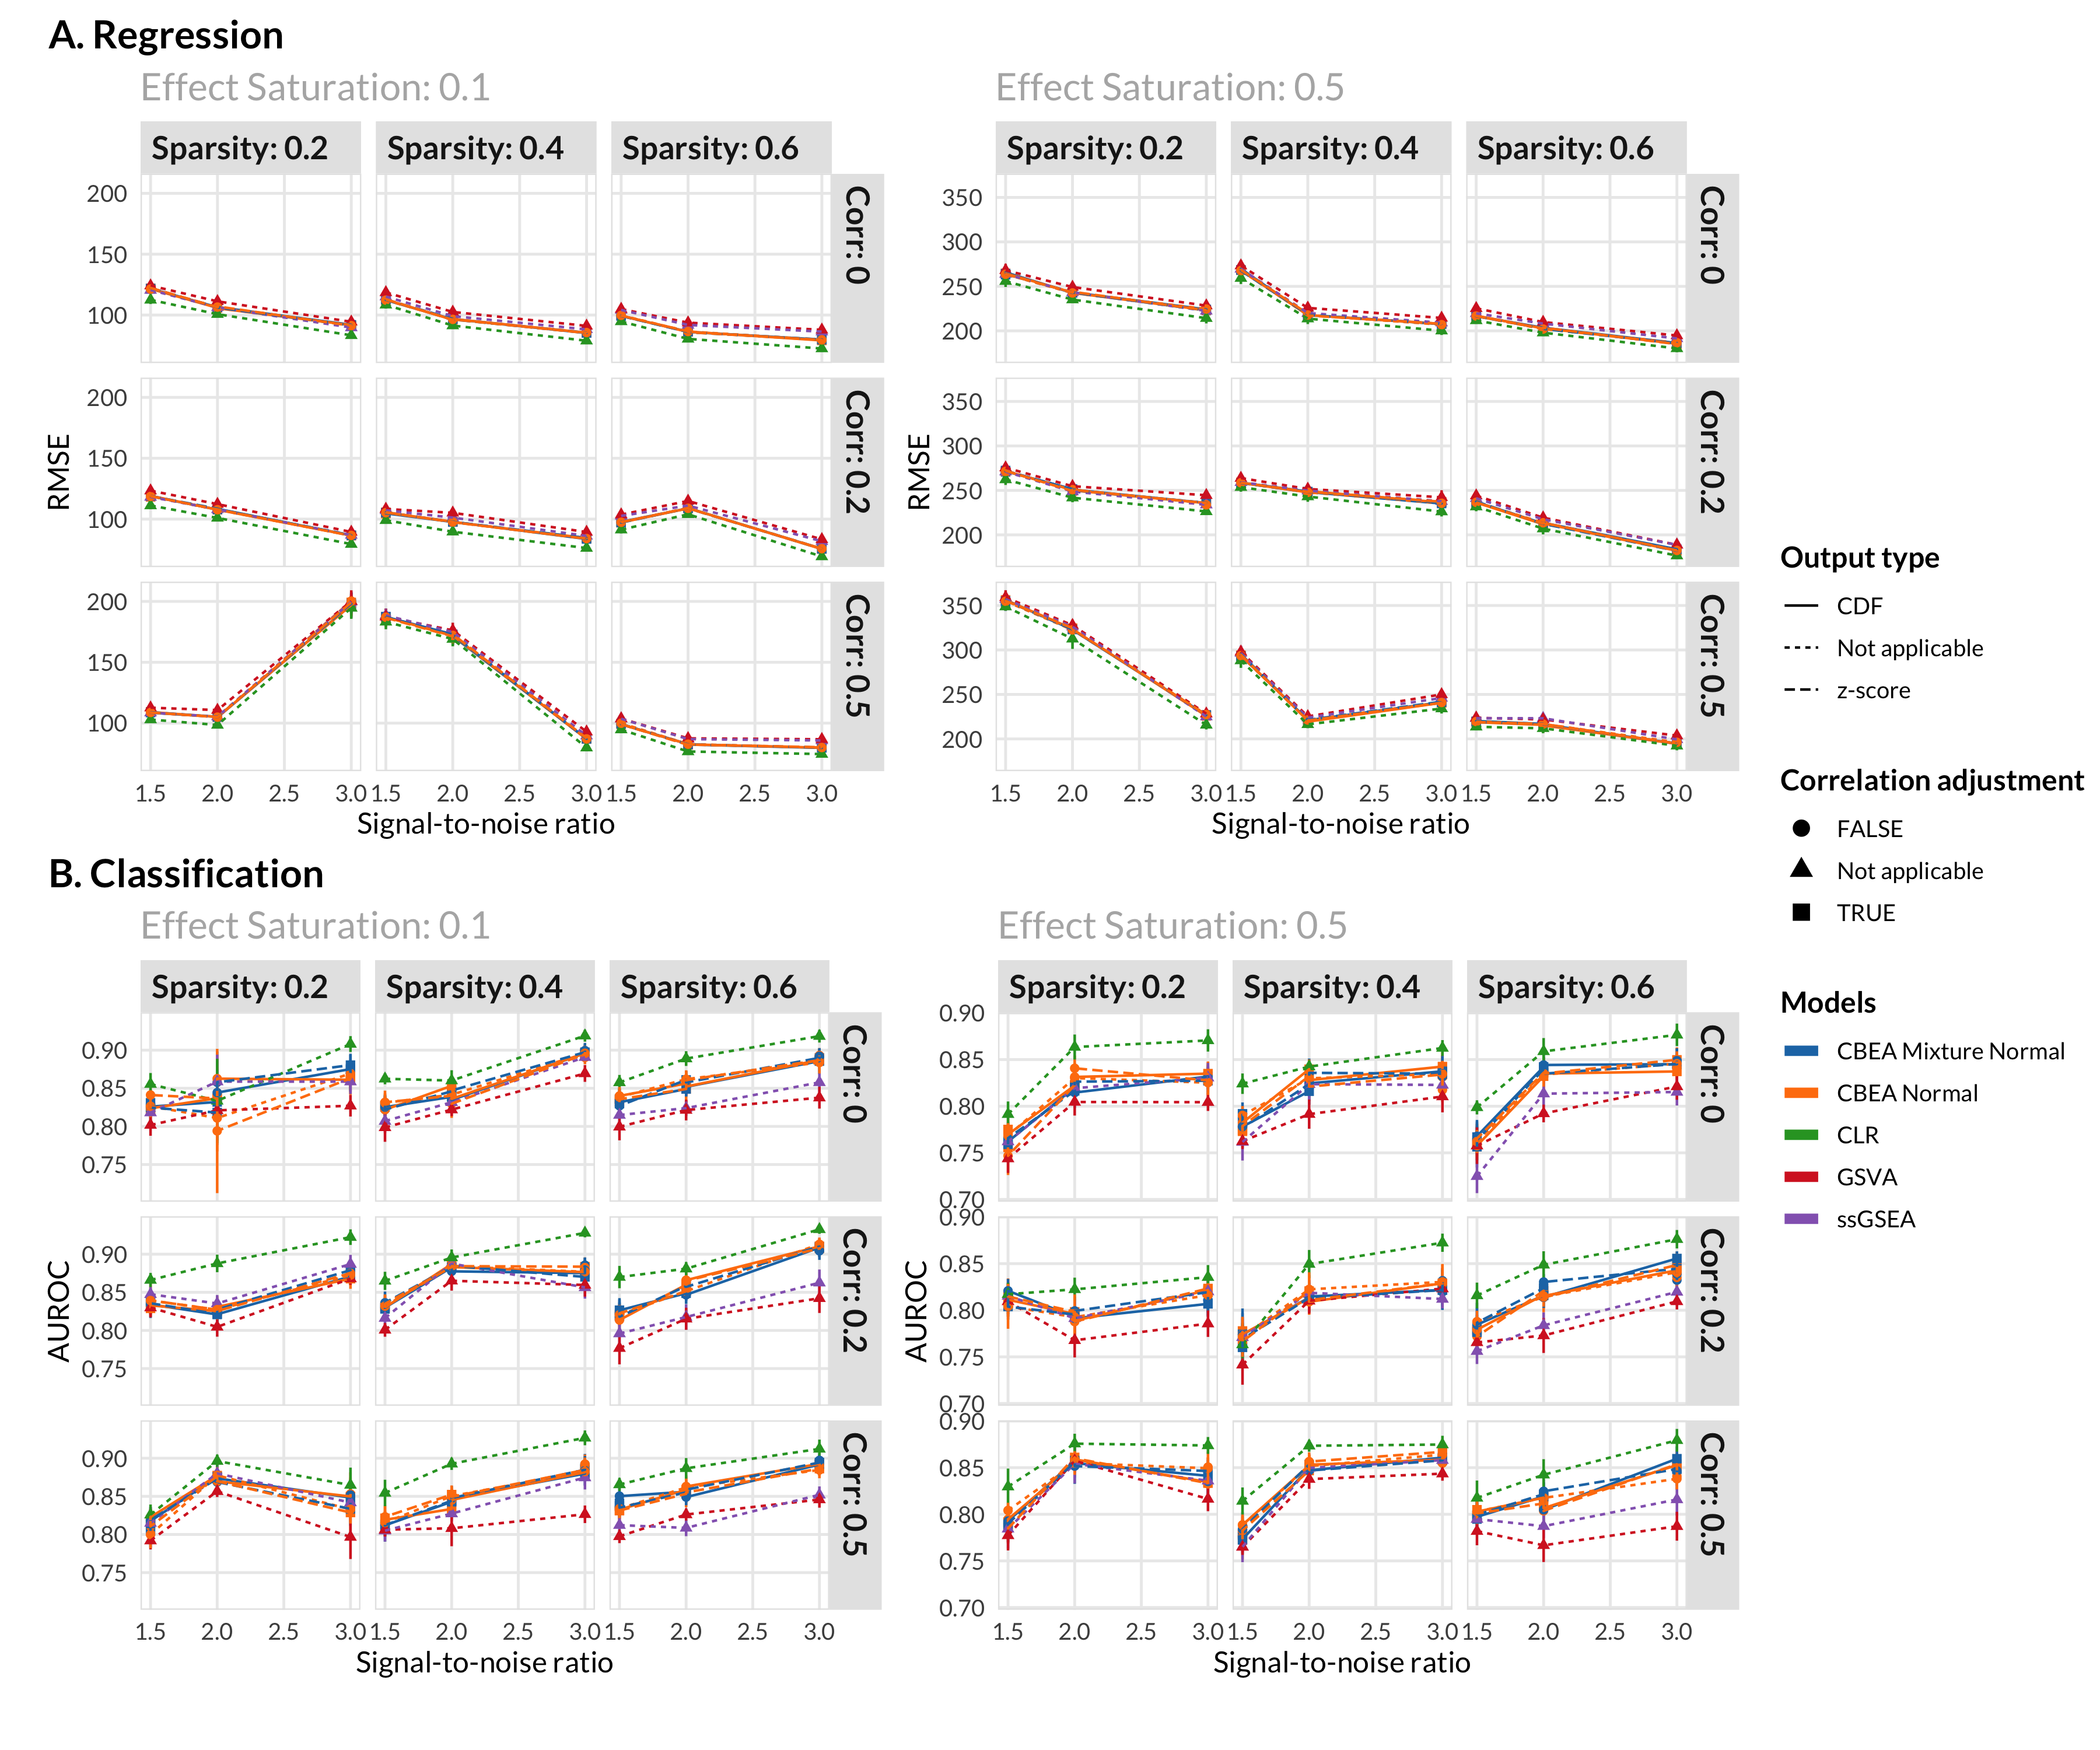
\includegraphics[width = \linewidth]{figures/sim_pred_combined.png}
    \caption{Predictive performance of a naive random forest model trained on CBEA, ssGSEA, GSVA generated scores as well as the standard CLR approach on simulated across different levels of data sparsity, inter-taxa correlation, effect saturation, and signal-to-noise ratio. Panel \textbf{(A)} presents performance on a regression task using predictive R-squared as the evaluation measure. Panel \textbf{(B)} presents performance on a classification task with AUC as the evaluation measure. CBEA approaches outperformed GSVA and ssGSEA across all simulation conditions but not the CLR approach.}
    \label{fig:6}
\end{figure}


%\begin{figure}[!ht]
%    \centering
%    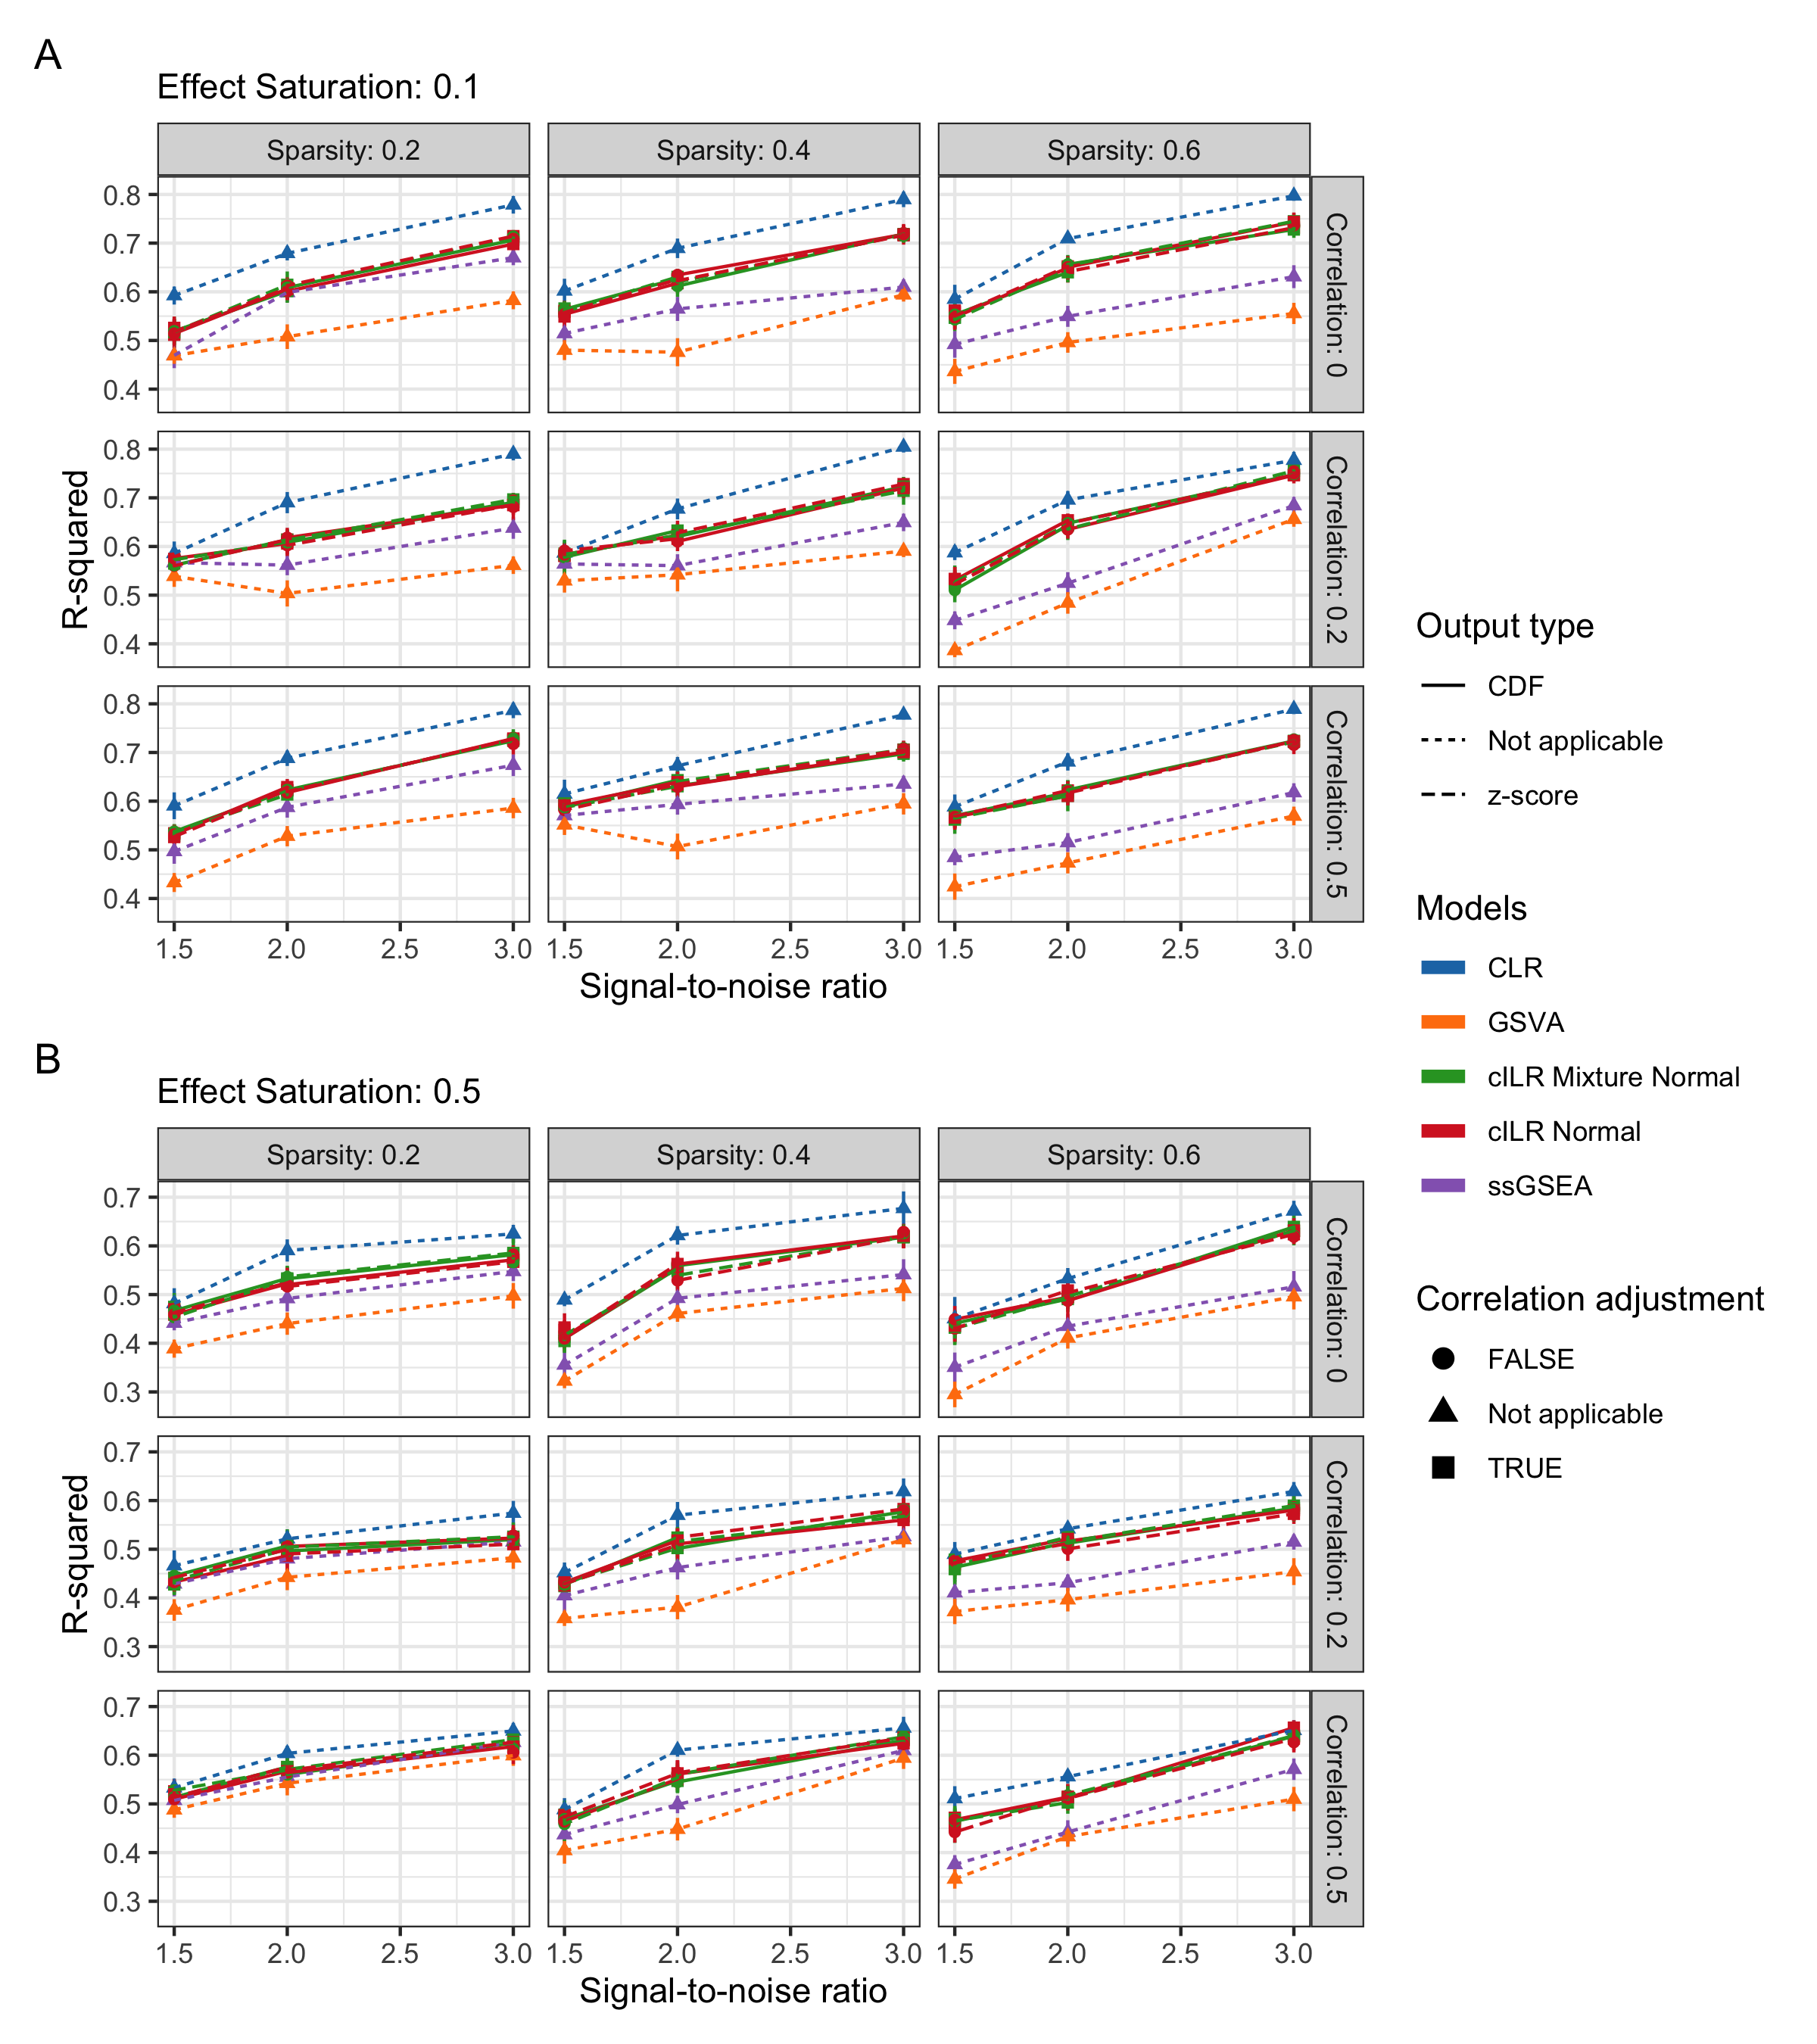
\includegraphics[width=\textwidth]{figures/sim_pred_rsq.png}
%    \caption{Predictive R-squared of a random forest model for a continuous outcome trained on CBEA,     %ssGSEA, GSVA generated scores as well as on standard CLR transformed data evaluated on simulated data %across sparsity levels, correlation, and signal-to-noise ratio. Panel \textbf{(A)} and \textbf{(B)} %represent results across different levels of model saturation (proportion of sets associated with the %outcome). CBEA approaches outperformed GSVA and ssGSEA but not standard CLR.}
%    \label{fig:sim_pred_rsq}
%\end{figure}

\subsubsection*{Real data evaluations}
In addition to parametric simulations, we also assessed the performance of using CBEA scores in predictive models with real data sets. Fig~\ref{fig:7} presents results for two data sets with a similar disease classification task of discriminating patients who are diagnosed with IBD (includes both Crohn's disease and ulcerative colitis) using only microbiome taxonomic composition. The two data sets represent different microbiome sequencing aprpaoches: the Gevers et al. \cite{gevers2014} data set uses 16S rRNA gene sequencing, while the Nielsen et al \cite{nielsen2014} data set uses whole genome shotgun sequencing. 

\begin{figure}[!h]
    \centering
    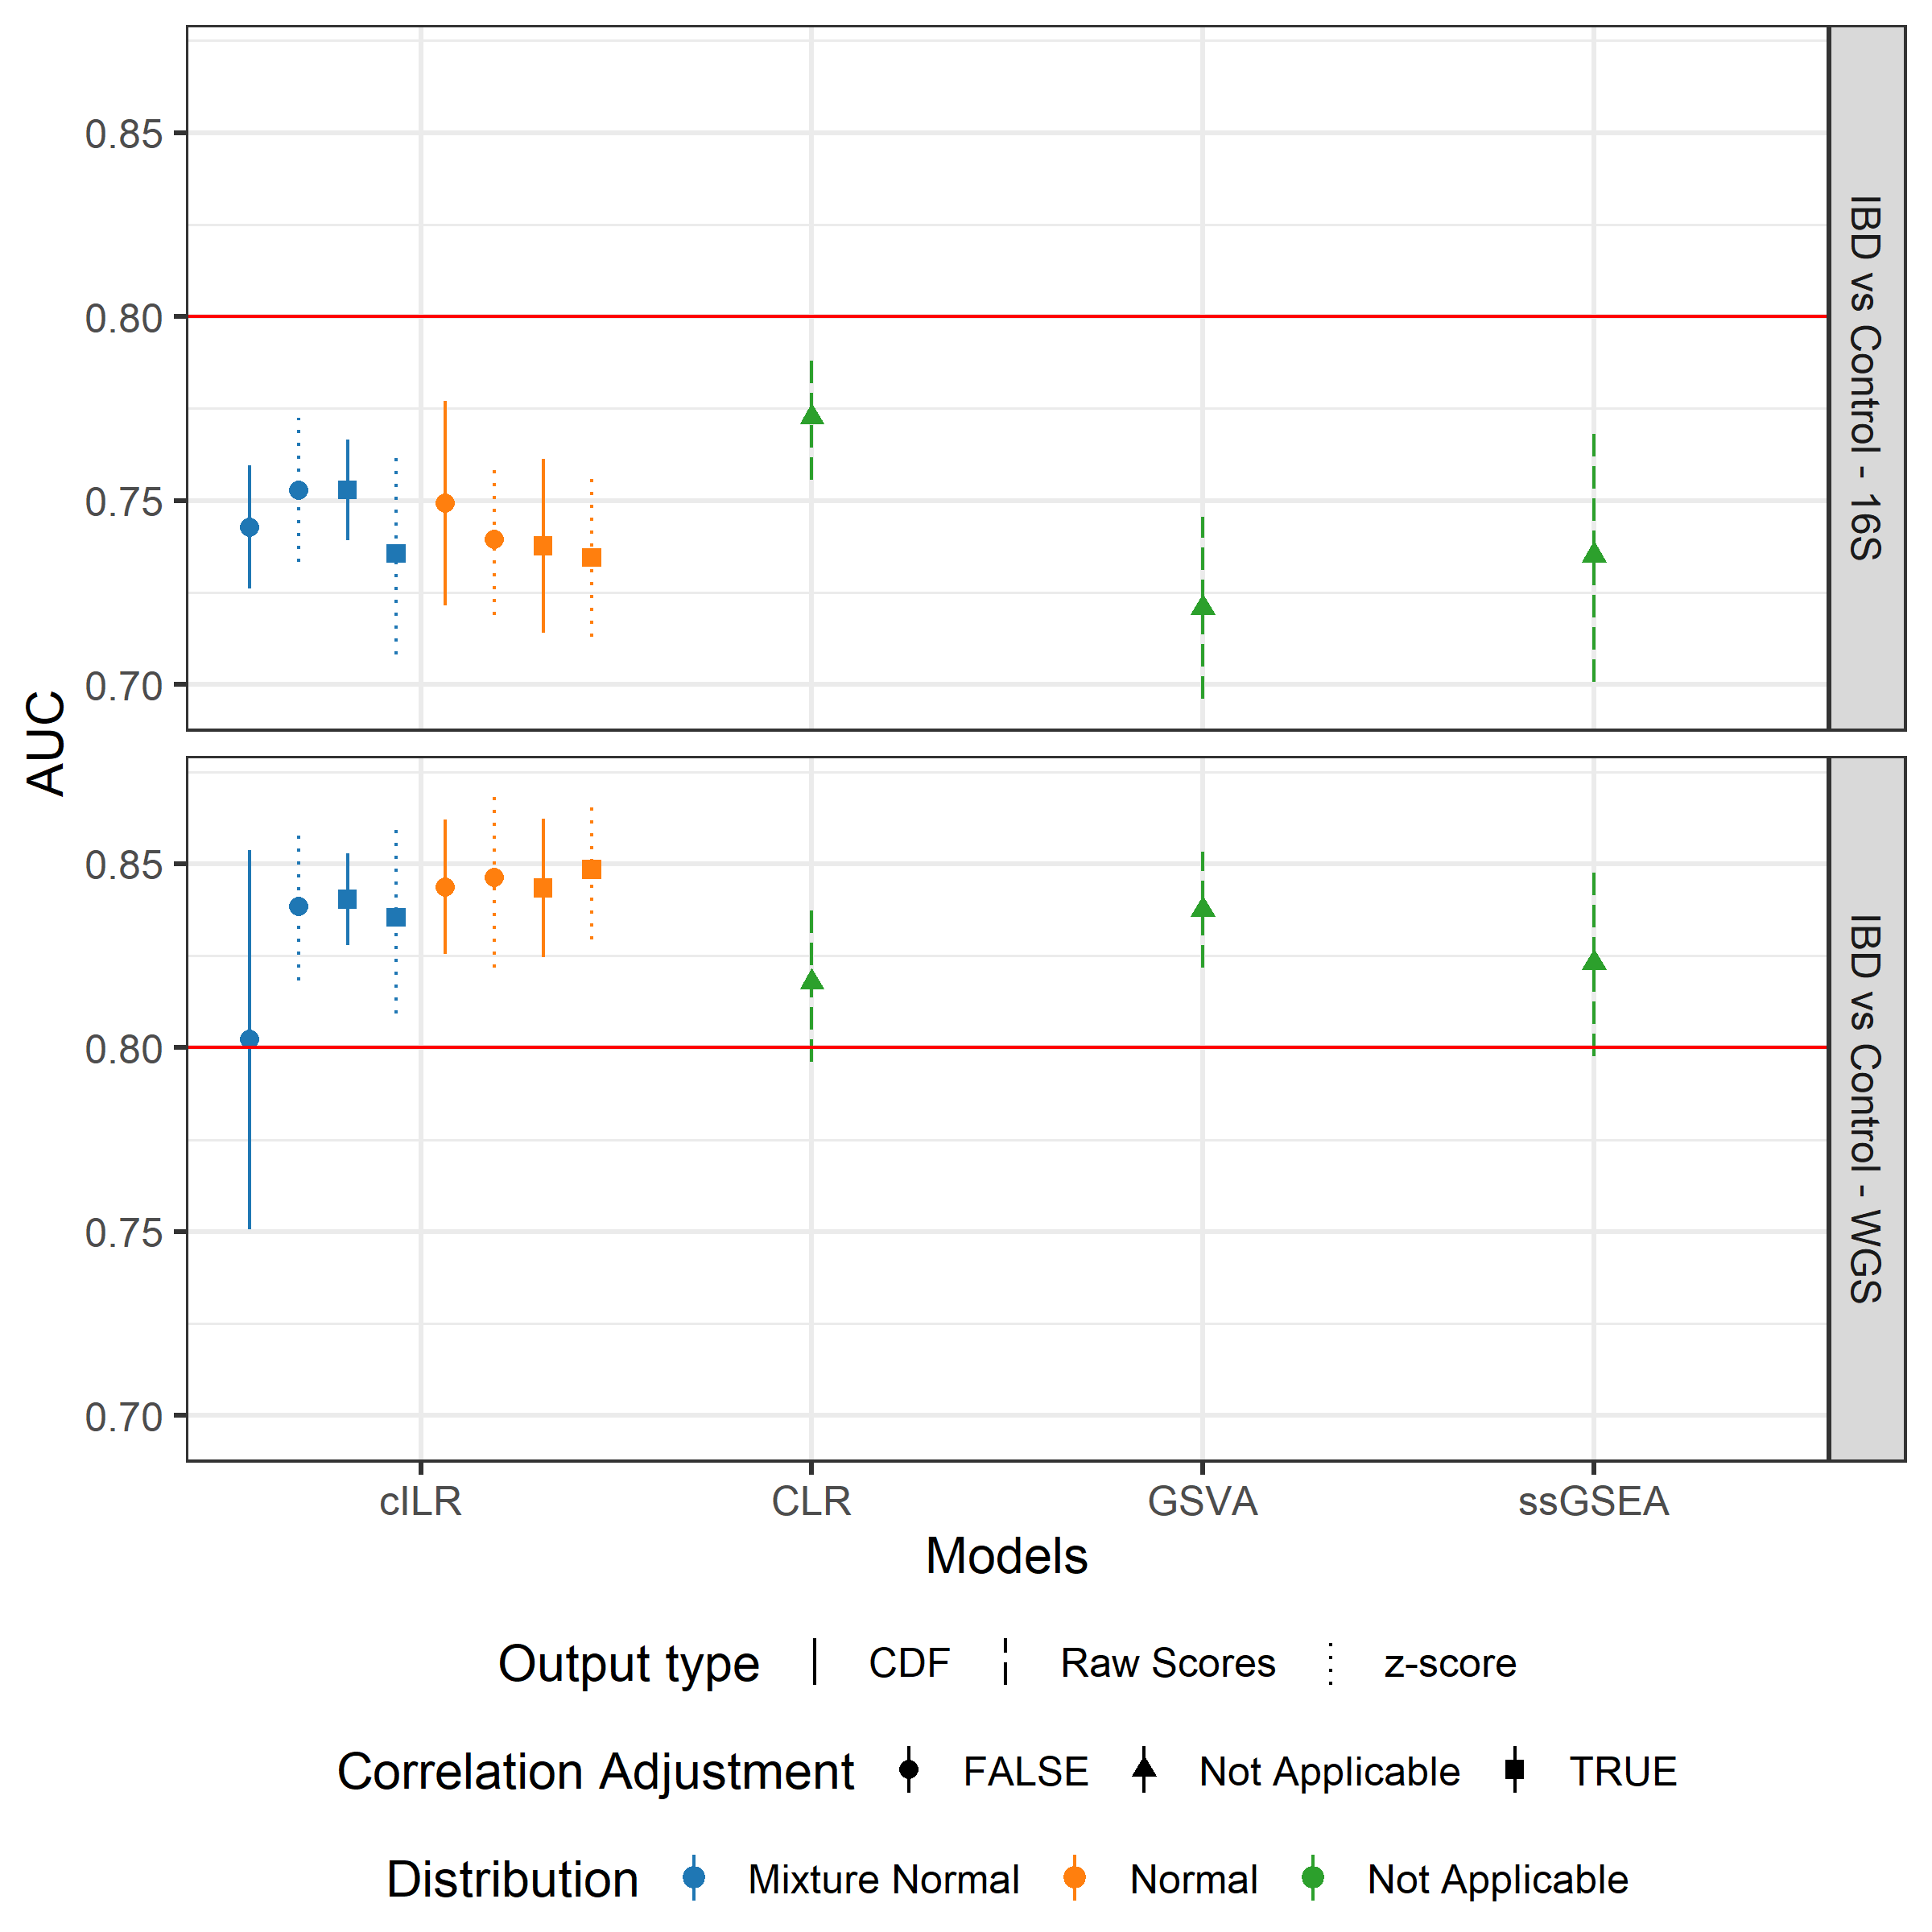
\includegraphics[width = \linewidth]{figures/data_prediction_plot.png}
    \caption{Predictive performance of a naive random forest model trained on CBEA, ssGSEA, GSVA generated scores as well as the standard CLR approach on predicting patients with inflammatory bowel disease versus controls using genus level taxonomic profiles. Data sets used span both 16S rRNA gene sequencing (Gevers et al. \cite{gevers2014}) and whole-genome shotgun sequencing (Nielsen et al. \cite{nielsen2014}). CBEA performs better than GSVA and ssGSEA but not as well as CLR, with the exception of the whole genome sequencing data set.}
    \label{fig:7}
\end{figure}

Similar to simulation experiments, we also fitted a naive random forest model using CBEA, ssGSEA, GSVA, or CLR transformed variables as inputs, and use AUC as the performance criteria. Results also replicated that of the simulations, where across both data sets CBEA and CLR methods provide much better performance than both GSVA or ssGSEA. Interestingly, the CBEA approach performed better than CLR in the whole genome data set but did not perform as well in the 16S rRNA gene sequencing data set. However, these results indicate that CBEA generated scores are informative, providing competitive performance when acting as inputs to disease predictive models. Most importantly, performance values are consistent across both simulated and real data sets. 

These results demonstrate that CBEA generated scores are informative features in disease prediction tasks. Simulation results indicate that CBEA methods perform much better than either GSVA or ssGSEA, but not as well as the standard CLR approach. Interestingly, however, CBEA methods were much more competitive with CLR in either WGS data sets or data sets with higher sparsity levels. 


\section*{Discussion}

\subsection*{Inference with CBEA}
The formulation of CBEA as a comparison between taxa within the set and its complement corresponds to the competitive null hypothesis in the gene set testing literature \cite{tian2005}. This allows for conducting inference with CBEA even at the sample-level. We assessed the usage of CBEA in this type of analysis by evaluating type I error and power across both simulation studies and real data applications. Most importantly, we demonstrated that our adjusted CBEA approach was able to address the issue of variance inflation due to correlation \cite{wu2012} by controlling for type I error at the appropriate $\alpha$ level across different levels of simulated inter-taxa correlation (Fig~\ref{fig:2}) while conversely unadjusted CBEA and the naive Wilcoxon rank sum test showed much higher rates of error. This is further encouraged in real data analysis where the false discovery rate was around $0.05$ when a collection of true null and true alternate hypotheses were tested. Unfortunately the trade-off of good type I error control is lower power. The conservativeness of the test attenuates with higher sparsity and correlation, where power was not approaching even 50\% even at the highest effect sizes. However, when the degree of such data features are reasonable, CBEA will still be able to detect a reasonable proportion of samples with inflated counts.  

We also observed that choosing different distributional forms did not alter performance values for CBEA. This runs contrary to our comparison analysis in Fig~\ref{fig:1}, where we demonstrated that the mixture normal distribution had superior fit compared to the simple normal for raw CBEA scores computed under the global null. We hypothesized that this might be due to the difficulty in fitting mixture distribution to data using the expectation maximization algorithm, as the convergence rate is slow when there is high overlap between the mixtures, resulting in a small mixing coefficient for one of the components \cite{naim2012}. As such, in our implementation of CBEA, in order to ensure convergence for the estimating procedure we increased the number of iterations while relaxing the tolerance parameter. Furthermore, there are also possible problems with our adjustment procedure for the mixture distribution that might impact overall fit. In order to combine the scale and location estimate of two mixture distributions, we fixed the overall mean, standard deviation, mixing coefficient and component-wise means and used an optimization procedure to find the component-wise variances. However, this means that we have one equation for the overall variance but two possible parameters to estimate. As such, there is no guaranteed unique solution to component-wise variances. We hypothesized that the instability and degeneracy in component-wise variance estimates might impact the fidelity of estimates at the tails of the distribution, thereby affecting inference.  

Despite these concerns, empirical results still indicate that CBEA can confidently identify samples with inflated counts. The conservativeness of the correlation adjustment procedure ensures that significant results can be trusted by practitioners, even if CBEA might not be able to exhaustively identify all samples with inflated counts. In situations where either the data is less sparse (e.g. containing a lot of core taxa that are prevalent across all samples), there is less inter-taxa correlation within the set (e.g. taxa that do not participate in common pathways but have shared characteristics like pathogenicity), or if the effect size is large, then CBEA will still be able to produce reasonable power. A practitioner can use CBEA to screen for samples for subsequent analysis that might involve significant costs, or perform hypothesis generation using a less stringent criteria alongside a multiple testing adjustment procedure (such as Benjamini-Hochberg \cite{benjamini1995}). 

\subsection*{Downstream analysis}
The sample-level enrichment scores generated by the CBEA method can be used in downstream analyses commonly performed in microbiome research: differential abundance testing and disease prediction.

\subsubsection*{Differential abundance analysis}
For differential abundance testing, we evaluated whether using CBEA scores alongside a standard difference in means test (Welch's t-test and Wilcoxon rank sum test) is suitable to detect changes in abundance of a set of microbes. We compared CBEA against two popular approaches: corncob \cite{martin2020} and DESeq2 \cite{love2014} applied on data where taxa were aggregated using the naive sum method. We chose DESeq2 because it is an older approach from the bulk RNA-seq literature that has strong support for usage in microbiome taxonomic data \cite{mcmurdie2014}. Conversely, corncob is a newer method developed specifically for microbiome taxonomic data sets, where taxonomic counts are modeled directly using a beta-binomial distribution instead of relying on normalization via size factor estimation like in DESeq2. 

Surprisingly, we found some conflicting results when evaluating comparisons across parametric simulations and real data analysis. The performance of CBEA was consistent across two evaluation criteria, demonstrating good type I error and respectable power. However, corncob and DESeq2 showed opposite effects: in simulation experiments, both methods show good type I error control but low power, while in real data analyses, conversely both corncob and DESeq2 showed inflated type I error but comparable power with respect to CBEA methods. Despite such discrepancy, results still indicate good performance of CBEA scores when used as inputs to downstream differential abundance analysis compared to using aggregated raw counts, even in methods designed to handle that type of data such as corncob and DESeq2.

We hypothesized that the above behavior can arise due to issues with performing inference in the presence taxon-specific protocol biases \cite{mclaren2019}. According to McLaren et al., the observed relative abundance of taxa is different than the true relative abundance due to protocol bias, and importantly this bias is specific to each taxon \cite{mclaren2019}. This is especially true in the context of sum-based aggregations, where the resulting bias of the aggregated taxon are dependent on the relative abundances of the contributing taxa (Appendix I in \cite{mclaren2019}). Conceptually, this means that measurement error for a taxon aggregate is different across samples as relative abundance of contributing changes, leading to issues when attempting to perform inference. As such, we expect methods like corncob or DESeq2 when performed on such aggregates to have inflated type I error compared to our taxon-ratio based approach.  

The bias model also helps explain differences in performance of DESeq2 and corncob in simulation analyses compared to real data. Our simulation protocol does not explicitly include bias in our formulation, and all taxa were generated from the same underlying distribution with similar variances across all samples (the only difference is in the mean value where a taxa is expected to have inflated counts). As such, we do not expect our simulated taxa to have any taxon-specific biases, which is not the case in real data settings. Therefore, we can expect DESeq2 and corncob to retain their expected type I error control in simulation analyses compared to real data. It is still surprising to see lower power for both methods in simulation analyses, which might be due to the fact that the evaluation protocol only considers default settings for both methods and did not attempt to optimize performance. 

The fact that the performance of CBEA remains consistent across both simulation and real data analysis shows that CBEA is invariant to taxon-specific biases. Furthermore, our evaluation indicates that even a simple difference in means test when used in combination with CBEA scores can preserve type I error while maintaining good power. As such, a practioner can use CBEA as a pre-processing step prior to performing a differential abundance test.  

\subsubsection*{Predictive models}
For disease prediction, we fitted a basic random forest model \cite{breiman2001} to predict continuous and binary outcomes using CBEA generated scores as inputs. Similar to our inference analysis, we compared CBEA against both ssGSEA and GSVA. Additionally, we also evaluated CBEA with the approach where counts of a set were aggregated using sums and then centered log-ratio transformed. This is because CLR is considered standard practice in using microbiome variables as predictors for a model \cite{gloor2017}. Results indicated that CBEA produces good performance values across both real data analysis and simulation scenarios. Since predictive models consider the effect of variables jointly (and in the case of random forest, consider interactions as well), good performance indicates that CBEA scores can capture joint distribution of sets, enabling both uniset and multi-set type analyses. Comparatively, CBEA generated scores outperformed other enrichment score methods (GSVA and ssGSEA), suggesting that it is more tailored for microbiome taxonomic data sets. This is consistent with our sample ranking analysis (Fig~\ref{fig:3}), where CBEA scores are on average more informative when used to rank samples based on their propensity to have inflated counts. However, CBEA did not outperform the CLR approach across our simulation studies, and only marginally performed better in the real data analysis with WGS data. 

However, in simulation studies, this performance gap between CLR and CBEA decreases with higher sparsity and correlation, especially in low effect saturation scenarios. Additionally, there are also downsides to applying CLR. First, the singular covariance matrix of CLR transformed variables is singular due to a sum to zero constraint \cite{gloor2017}, preventing the proper usage of approaches that rely on matrix decomposition. Second, the procedure still relies on using summation of counts prior to transformation, which means that we still can't compare across sets of different sizes, and any bias might still be propagated \cite{mclaren2019}. As such, despite benefits in performance for a naive random forest model, there is still space for using CBEA as primary inputs into predictive models. 

Similar to other experiments in downstream usage of CBEA, performance did not change with different underlying distributions, output types, or correlation status. This is surprising since we expect z-scores to perform better as they are able to capture the direction of an association. The fact that this effect persisted even onto our real data analysis suggests that this is not due to a deficiency of our simulation design. As such, practitioners who wish to use CBEA in predictive models might be suited to use the settings that is the fastest to compute.  

Ultimately, results indicate that CBEA can produce informative scores that contribute to competitive performance of prediction models even in low signal-to-noise ratios with high inter-taxa correlation and sparsity. Even though there exists situations where it might not provide maximum predictive values, the flexibility of CBEA in various types of analyses enable even though in some scenarios it might not provide maximum predictive values. 

\subsection*{Limitations and future directions} 
There are various limitations to our evaluation of CBEA. First, our simulation analysis might not capture the appropriate data-generating distributions underlying microbiome taxonomic data. There is strong evidence to suggest that our zero-inflated negative binomial distribution is representative \cite{calgaro2020}, however other distributions such as the Dirichlet multinomial distribution \cite{wu2016} have been used in the evaluation of prior studies. Second, the usage of the gingival data set similar to \cite{calgaro2020} to assess power in differential abundance testing and single sample inference is not perfect. This is because the oxygen usage label of each microbe in the data set is only available at the genus level, and the difference in counts for obligate aerobes and anaerobes across the supragingival and subgingival sites might not be as clear cut. As such, results from power analyses using this data set is only relative between the comparison methods. Finally, we assumed that taxa within a set are all equally associated with the outcome. This limits our ability to evaluate the performance of CBEA when only a small number of taxa within the set is associated with the outcome, or if there are variability in effect sizes or association direction of taxa within a set. 

Our evaluation showed various drawbacks of the CBEA method. First, inference with CBEA is limited in being able to exhaustively detect all samples with significant inflated counts for a set in situations where there is a high degree of sparsity and inter-taxa correlation. Second, for downstream analyses, CBEA might not always perform better than competing methods, especially when being used to generate inputs to predictive models. We hypothesized that this might be due to the lack of fit for the underlying null distribution in high correlation settings, especially the identifiability problem associated with adjusting the mixture normal distribution. As such, we hope to refine the null distribution estimating procedure by either choosing a better distributional form, or to further constrain the optimization procedure of the mixture normal distribution by fixing the third and fourth moments. 

In addition, there are possible extensions CBEA can we can consider to provide more flexibility across different data analysis scenarios in data analysis. First, CBEA did not address the sparsity of microbiome taxonomic data and relies on a pseudocount to ensure log operations are valid. We can address this by incorporating more sophisticated model-based zero-correction methods such as in \cite{martin-fernandez2012} or \cite{kaul2017a}. Second, CBEA also treated all taxa within the set as equally contributing to the set. Incorporation of taxa-specific weights could reduce the influence of outliers, such as rare or highly invariant taxa. Finally, curating sets based on \emph{apriori} characteristics of microbes can allow for incorporating functional insights into microbiome-outcome analyses while also improving interpretability when compared to using taxonomic categories such as phylum or genus alone.  

\section*{Conclusion}
Gene set testing, or pathway analysis is an important tool in the analysis of high-dimensional genomics data sets. However, limited work has been done developing set based methods specifically for microbiome relative abundance data. We introduced a new microbiome-specific method to generate set-based enrichment scores at the sample level. We demonstrated that our method can control for type I error for significance testing at the sample level, while generated scores are also valid inputs in downstream analyses, including disease prediction and differential abundance.  

\section*{Acknowledgments}
The authors thank Becky Lebeaux, Modupe Coker, Erika Dade, Jie Zhou, and Weston Viles for insightful comments and suggestions that greatly improved the paper. 

\nolinenumbers
% Either type in your references using
% \begin{thebibliography}{}
% \bibitem{}
% Text
% \end{thebibliography}
%
% or
%
% Compile your BiBTeX database using our plos2015.bst
% style file and paste the contents of your .bbl file
% here. See http://journals.plos.org/plosone/s/latex for 
% step-by-step instructions.
% 

\bibliography{references}{}



\section*{Supporting information}

% Include only the SI item label in the paragraph heading. Use the \nameref{label} command to cite SI items in the text.
\paragraph*{S1 Fig.}
\label{S1_Fig}
{\bf Computational performance of CBEA.} Computational time (in seconds) as a function of sample size (left panel) and number of taxa sets evaluated (right panel). Evaluation was performed on simulated data sets. For sample size analysis, only 10 sets were evaluated. For taxa set analysis, sample size was fixed at 1,000. Across all evaluations, the size of each taxa set was also fixed at 50. 

\paragraph*{S2 Fig.}
\label{S2_Fig}
{\bf Distribution of p-values.} Q-Q plot of 10,000 p-values compared against a uniform distribution bounded between 0 and 1. Evaluation was performed on simulated null data sets of 10,000 samples testing for enrichment of a set of size 50. For correlation of 0.5, p-values represent correlation adjusted CBEA while for correlation of 0, p-values represent unadjusted CBEA. 

\paragraph*{S1 File.}
\label{S1_File}
{\bf Supplemental derivations.} Includes additional details on addressing variance inflation due to correlation in CBEA, as well as computational performance and p-value distribution of the method.   

\end{document}

